%%%%%%%%%%%%%%%%%%%%%%%%%%%%%%%%%%%%%%%%%%%%%%%%%%%%%%%%%%%%%%%%%%%%%%%%%%

% abnTeX2: Modelo de Trabalho Acadêmico em conformidade com 
% as normas da ABNT

%%%%%%%%%%%%%%%%%%%%%%%%%%%%%%%%%%%%%%%%%%%%%%%%%%%%%%%%%%%%%%%%%%%%%%%%%%

\documentclass[english, 
               brazil, 
               bsc] %Opções bsc (TCC) e msc (Mestrado)
               {dcomp-abntex2}


%%%%%%%%%%%%%%%%%%%%%%%%%%%%%%%%%%%%%%%%%%%%%%%%%%%%%%%%%%%%%%%%%%%%%%%%%%
% Área para adição de pacotes extras
%%%%%%%%%%%%%%%%%%%%%%%%%%%%%%%%%%%%%%%%%%%%%%%%%%%%%%%%%%%%%%%%%%%%%%%%%%

\usepackage{lipsum} %Retirar para a versão final do documento

%Utilize aqui seu pacote preferido para algoritmos
\usepackage[linesnumbered]{algorithm2e}
\usepackage{tabularx}

%%%%%%%%%%%%%%%%%%%%%%%%%%%%%%%%%%%%%%%%%%%%%%%%%%%%%%%%%%%%%%%%%%%%%%%%%%

%Compila o indice
\makeindex

\begin{document}

% Seleciona o idioma do documento (conforme pacotes do babel)
\selectlanguage{brazil}

% Retira espaço extra obsoleto entre as frases.
\frenchspacing 

%%%%%%%%%%%%%%%%%%%%%%%%%%%%%%%%%%%%%%%%%%%%%%%%%%%%%%%%%%%%%%%%%%%%%%%%%%
% ELEMENTOS PRÉ-TEXTUAIS
%%%%%%%%%%%%%%%%%%%%%%%%%%%%%%%%%%%%%%%%%%%%%%%%%%%%%%%%%%%%%%%%%%%%%%%%%%

\pretextual

\titulo{Proposta de Aplicação Móvel para Autocuidado de Diabéticos com Acuidade Visual Prejudicada} 
\autor{Jonathan Kelvin de Jesus Santos}
\orientador{Profa. Dra. Adicinéia Aparecida de Oliveira}
\curso{Sistemas de Informação}

\inserirInformacoesPDF

\imprimircapa
% \imprimirfolhaderosto*

% \begin{dedicatoria}
   \vspace*{\fill}
   \centering
   \noindent
   \textit{Este trabalho é dedicado a todos que acreditam na educação\\
   como meio essencial para o desenvolvimento sustentável de qualquer sociedade.} \vspace*{\fill}
\end{dedicatoria}
% ---
%\begin{agradecimentos}

Não haveria como não falar da minha mãe, Diana, em primeiro lugar neste espaço,
esta que abriu mão de diversas coisas para lutar pelo bem de seus 3 filhos, que sempre quis o melhor
pra mim e fez o que pôde para evitar e alertar sobre meus erros. E mesmo não entendendo minhas escolhas,
não as barrou e sempre esteve lá para quando eu quebrasse a cara.

Mãe, obrigado por tudo!

Agradeço também à Sergiane e Walesson, que me confiaram a honra de ser padrinho de Walace.
Aos meus irmãos Daiane e David que, em meio à tantas brigas, sempre nos apoiamos e defendemos uns aos outros.
Ao meu primo, Lucas, que foi uma referência durante a graduação. E, ao restante dessa grande família que, embora
não os nomeie aqui, quero que saibam que foram e são muito importantes para mim.

As amizades que fiz foi o que me manteve firme para seguir até o final dessa jornada. Assim, não posso deixar de mencionar
Abayomi com quem tenho quilômetros de mensagens trocadas no Telegram e que está em constante mudança e revolta (\emph{pelu idi}).
Brunna que talvez não saiba, mas nos momentos em que eu estava cheio de ansiedade, fez-me sentir em paz,
enquanto lia livros no silêncio de sua sala.

Igor e seus argumentos socráticos que foram interpretados como sofistas e Geovanne que está trabalhando feito louco e
me deixando preocupado com um \emph{burnout}. Mayara que sempre notava quando estava desanimado e estava lá para quando
eu precisasse desabafar. Raul de quem eu tinha que esconder a preocupação para evitar que infartasse e, por fim devido
à ordem alfabética, Roberto, o tiozão do pavê.

Embora eu consciência de minhas dificuldades para me expressar, principalmente com relação a sentimentos,
não sei o por que, mas nunca consegui dizer ``Eu te amo'' para ninguém depois que cresci, nem mesmo para minha mãe.
Assim, queria aproveitar esse momento para aqui deixar registrado que embora nunca tenha-os dito:

Amo vocês!

Não posso esquecer dos professores do DComp que apresentaram os caminhos que possibilitaram que eu seguisse nessa jornada.
Também aos professores de outros departamentos como o DPS e DCS que mostraram a importância do pensamento crítico.
E, em especial, a Gilton sempre animado e com novas ideias, Leonardo por seus conselhos e desafios, e Ricardo que nos ouvia
e parecia entender nossas frustrações.

E, por fim, à minha orientadora Adicinéia que, além da orientação e paciência comigo neste trabalho,
foi a única que, transmitindo conhecimento durante as aulas, conseguiu manter minha concentração por tanto tempo,
horas, sem me dar sono.

\end{agradecimentos}
% ---
%\begin{epigrafe}[]
    \vspace*{\fill}
	\begin{flushright}
	
		\textit{Num processo de construção, de capital\\
				Esquecemos de algo vital, a inclusão\\
				E promovemos a exclusão, digital\\
				}
		
	\end{flushright}
\end{epigrafe}
% ---
%% resumo em português
\setlength{\absparsep}{18pt} % ajusta o espaçamento dos parágrafos do resumo
\begin{resumo}
    O \emph{Diabetes Mellitus} (DM) é um grupo de doenças endocrinológicas crônicas caracterizado pela elevação
    da glicose no sangue que requer cuidados médicos contínuos para redução de risco e controle glicêmico, e vem se
    tornando um desafio cada vez maior devido ao rápido aumento do número de casos nos últimos 20 anos. Com isso,
    complicações do DM já são a maior causa de cegueira em adultos de países desenvolvidos, sendo que pelo menos 2,2
    bilhões de pessoas no mundo vivem com deficiência visual (DV) em algum grau.
    Estudos anteriores identificaram a importância do autocuidado no tratamento do DM, a dificuldade
    no acesso a informações a respeito por pacientes com DV e as principais funcionalidades utilizadas
    como solução no mercado. Além disso, neste trabalho foi constatado que, mesmo com o aumento da informatização e
    popularização dos \emph{smartphones}, pessoas com DV ainda enfrentam sérias dificuldades devido à falta
    de acessibilidade em aplicações móveis. Perante o exposto, foi realizado um processo de Mapeamento Sistemático da
    Literatura (MSL) para estabelecer as técnicas de acessibilidade que poderiam ser adotadas no desenvolvimento
    de um aplicativo móvel chamado DiaVision. Assim, o aplicativo foi desenvolvido para Android e iOS, atendendo
    aos requisitos identificados para este público-alvo e soluções de acessibilidade encontradas no MSL\@.
    Uma versão inicial do \emph{app} foi avaliada por 77 pacientes com DV e os resultados desse estudo
    mostraram que 90,1\% dos participantes gostariam de ter o \emph{app}, com 62,3\% avaliando-o com nota máxima.
    Contudo, parte das soluções de acessibilidade foram implementadas após a realização desse estudo, assim,
    35,1\% dos participantes apontaram que o aplicativo precisava de melhorias quanto à acessibilidade. Dessarte,
    trabalhos futuros devem realizar uma nova avaliação do aplicativo com as novas funcionalidades e melhorias
    relativas à acessibilidade.

    \textbf{Palavras-chave}: aplicativo móvel. diabetes mellitus. autocuidado. acessibilidade. deficiência visual.
\end{resumo}
%% resumo em inglês
\setlength{\absparsep}{18pt} % ajusta o espaçamento dos parágrafos do resumo
\begin{resumo}[Abstract]
  \begin{otherlanguage*}{english}
    Diabetes Mellitus (DM) is a group of chronic endocrine diseases characterized by elevated blood
    glucose that requires continuous medical care for risk reduction and glycemic control, and has become
    an increasing challenge due to the rapid increase in the number of cases in the last 20 years. As a result,
    complications from DM are already the leading cause of blindness in adults in developed countries, with at
    least 2.2 billion people in the world living with visual impairment (VI) to some level. Previous studies
    have identified the importance of self-care in the treatment of DM, the difficulty in accessing information
    about it by patients with VI and the main features used as a solution in the market. Furthermore, in this
    work it was found that even with the increase in computerization and popularization of smartphones,
    people with VI still face serious difficulties due to the lack of accessibility in mobile applications.
    Therefore, a Systematic Literature Mapping (SLM) process was carried out to establish accessibility
    techniques that could be adopted in the development of a mobile application called DiaVision. Thus,
    the application was developed for Android and iOS, meeting the requirements identified for this target
    audience and accessibility solutions found in SLM\@. An initial version of the app was
    evaluated by 77 patients with VI and the results of this study showed that 90.1\% of the participants
    would like to have the app, with 62.3\% evaluating it with full mark. However, part of the
    accessibility solutions were implemented after this study was carried out, so 35.1\% of the
    participants pointed out that the application needed improvements in terms of accessibility. With
    this, future works must carry out a new evaluation of the application with the new functionalities
    and improvements related to accessibility.

    \textbf{Keywords}: mobile app, diabetes mellitus, self-care, accessibility, visual impairment.
  \end{otherlanguage*}
\end{resumo}


\mostrarlistadeILUSTRACOES
\mostrarlistadeQUADROS
\mostrarlistadeTABELAS
%\mostrarlistadeCODIGOS
%\mostrarlistadeALGORITMOS
 
% Lista de abreviaturas e siglas

\begin{siglas}
  	\item[API]{\textit{Application Programming Interface}}
  	\item[DCOMP]{Departamento de Computação}
  	\item[DM]{\textit{Diabetes Mellitus}}
  	\item[\emph{Dev}]{\textit{Developer}}
  	\item[DV]{Deficiência Visual}
  	\item[DVP]{Deficiência Visual Parcial}
  	\item[DVT]{Deficiência Visual Total}
  	\item[eMag]{Modelo de Acessibilidade em Governo Eletrônico}
  	\item[IBGE]{Instituto Brasileiro de Geografia e Estatística}
  	\item[OMS]{Organização Mundial da Saúde}
  	\item[PDV]{Pessoa(s) com Deficiência Visual}
  	\item[TA]{Tecnologias Assistivas}
  	\item[TTS]{\textit{Text-to-speech}}
  	\item[SO]{Sistema Operacional}
	\item[UFS]{Universidade Federal de Sergipe}
  	\item[UX]{\textit{User Experience}}
  	\item[WHO]{\textit{World Health Organization}}
  	\item[W3C]{\textit{World Wide Web Consortium}}
\end{siglas}
%\include{Pre_Textual/Simbolos}
    
\mostrarSUMARIO

%%%%%%%%%%%%%%%%%%%%%%%%%%%%%%%%%%%%%%%%%%%%%%%%%%%%%%%%%%%%%%%%%%%%%%%%%%
% ELEMENTOS TEXTUAIS
%%%%%%%%%%%%%%%%%%%%%%%%%%%%%%%%%%%%%%%%%%%%%%%%%%%%%%%%%%%%%%%%%%%%%%%%%%

\textual
%\chapter{Introdução}

% ---
\section{Contextualização e Motivação}
% ---

O Diebetes Mellitus (DM) vem se tornando um desafio global de saúde pública cada vez maior por conta do rápido aumento no número de casos nos últimos
20 anos \cite{ADA2019}.
Estimativas da Federação Internacional de Diabetes (IDF), do Atlas da Diabetes\footnote{\url{https://diabetesatlas.org/}}
de 2019, apontaram que 463 milhões de pessoas no mundo viviam com DM, o que representa cerca de 9.3\% da população
global adulta, e é esperado um aumento para 10,2\% (578 milhões) em 2030 e 10,9\% (700 milhões) em 2045 \cite{SAEEDI2019107843}.

O Brasil é o 5º país com mais diabéticos no mundo com 16,8 milhões em 2019, na faixa etária de 20 à 79 anos, e estimativas
de 21,5 e 26 milhões de casos para 2030 e 2045, respectivamente \cite{SAEEDI2019107843}. Os custos totais de hipertensão, diabetes
e obesidade no Sistema Único de Saúde (SUS) alcançaram 3,45 bilhões de reais em 2018, sendo 30\% desse custo relacionado ao DM \cite{Nilson2020}.

Já a retinopatia diabética é uma complicação vascular do diabetes, cuja prevalência está diretamente relacionada à duração
do diabetes e ao controle do nível de glicemia \cite{Solomon412}. Essa complicação é a maior causa de novos casos de cegueira
em adultos, na faixa etária de 20 à 74 anos, em países desenvolvidos \cite{ADA2019}. Além disso, outros distúrbios oculares
como o glaucoma e a catarata ocorrem mais cedo e com maior frequência em diabéticos \cite{ADA2019}.

Assim, atualmente o mundo enfrenta um sério problema com relação a saúde da visão. Segundo a Organização Mundial da Saúde (OMS),
pelo menos 2,2 bilhões de pessoas no mundo vivem com deficiência visual (DV) em algum grau, com isso,
a necessidade de cuidados com os olhos tende a crescer drasticamente nas próximas décadas \cite{WHO2019}.

Segundo a Associação Americana de Diabetes (ADA), serviços de educação e apoio para o autogerenciamento do diabetes
(DSMES, do inglês \emph{diabetes self-management education and support}) facilitam na aquisição de conhecimento e habilidades
necessárias para o autocuidado, incorporando as necessidades, objetivos e experiências de diabéticos \cite{ADA2019}. Portanto, DSMES
visam auxiliar o empoderamento dos pacientes com diabetes na tomada de decisões informadas de autogerenciamento \cite{Marrero2013}.

De acordo com estimativas de 2019, mais de 5 bilhões de pessoas no mundo possuem dispositivos móveis, sendo mais da metade destes, \textit{smartphones}
\cite{Taylor2019}. Embora, segundo \citeonline{morris2017smartphone}, cerca de 84\% da população estadunidense com DV possua ou utilize telefone celular,
a taxa média de indivíduos que possuem nos países menos desenvolvidos é de apenas 61\% \cite{ITU_2021}.

No Brasil, a taxa de adultos que relataram possuir dispositivos móveis foi de 83\% no total e 60\% para \textit{smartphones},
sendo que, na faixa etária entre 18 e 34 anos, houve um aumento no número de proprietários de \textit{smartphones} de
61\% em 2015 para 85\% em 2018 \cite{Taylor2019}.

\citeonline{Yan2019} elaboram um estudo abrangente, realizado com 479 \textit{apps} de 23 categorias da
\emph{Google Play}, utilizando uma ferramenta automatizada, o IBM \textit{Mobile Accessibility Checker}
(MAC), para encontrar possíveis problemas com acessibilidade relacionadas à DV nesses \textit{apps},
categorizando-os em V (Violação), PV (Potencial Violação) e A (Alerta). Os resultados mostraram que 94.8\%, 97.5\% e 66.4\% dos apps continham problemas
relacionados à V, PV e A, respectivamente \cite{Yan2019}.

Diante da popularização dos \emph{smartphones} e das problemáticas mencionadas, o presente trabalho visa desenvolver uma aplicação móvel
com DSMES, para ao autocuidado de diabéticos, considerando a resolução dos principais problemas de acessibilidade para pessoas com
deficiência visual (PDV).

% ---
\section{Objetivos}
% ---

Nesta seção são apresentados os objetivos, divididos em geral e específicos. Onde o objetivo geral dá uma visão mais ampla sobre o objeto
de estudo e os específicos visam aprofundar as intenções expressas no geral \cite{cervo2006metodologia}.

% ---
\subsection{Geral}
% ---

O objetivo deste trabalho é desenvolver uma aplicação móvel multiplataforma e assistiva voltada ao autocuidado de pessoas com diabetes
e acuidade visual prejudicada. Implementando soluções para os principais problemas de acessibilidade à PDV na utilização de aplicativos móveis.

% ---
\subsection{Específicos}
% ---

Para atingir objetivo deste trabalho, os seguintes objetivos específicos foram definidos:

\begin{itemize}
    \item Identificar os principais problemas enfrentados por PDV na utilização de aplicações móveis;
    \item Identificar as principais técnicas e soluções de acessibilidade à PDV para aplicações móveis;
    \item Relacionar as principais técnicas e soluções identificadas aos principais problemas identificados;
    \item Realizar o desenvolvimento do aplicativo móvel com os principais requisitos levantados;
    \item Aplicar as soluções identificadas para os principais problemas de acessibilidade ao aplicativo.
\end{itemize}

% ---
\section{Metodologia}
% ---

A metodologia adotada neste estudo foi a quantitativa exploratória, visando responder as questões de pesquisa apresentadas
no início do capítulo 3, assim, obtendo maior familiaridade com o problema e possíveis soluções.

Para isso, foi realizado um levantamento bibliográfico por meio de um Mapeamento Sistemático da Literatura (MSL), onde foi possível
realizar uma análise dos resultados dos estudos selecionados (de acordo com o protocolo) e dos relacionados (estudos de mapeamento).

% ---
\section{Organização do Documento}
% ---
Neste capítulo foram apresentados a contextualização, a motivação e os objetivos deste trabalho. Bem como, a metodologia adotada.

Para facilitar a navegação e melhor entendimento, este documento está organizado em capítulos, cujas descrições são listadas a seguir:
\begin{itemize}
    \item Capítulo 2 - Fundamentação Teórica: aborda os principais conceitos relacionados ao trabalho realizado;
    \item Capítulo 3 - Mapeamento Sistemático da Literatura: descreve os estudos selecionados e os relacionados, e apresenta uma análise dos resultados;
    \item Capítulo 4 - Plano de continuidade: descreve o que será realizado e apresenta o cronograma das próximas etapas deste trabalho.
\end{itemize}

%\chapter{Fundamentação Teórica}

Neste capítulo...

% ---
\section{Diabetes Mellitus}
% ---

De acordo com a Associação Americana de Diabetes (ADA), o Diabetes Mellitus (DM) é um grupo de doenças endocrinológicas crônicas
caracterizado pela elevação da glicose no sangue, devido à deficiência de ação do hormônio insulina, que requer cuidados médicos
contínuos para redução de risco e controle glicêmico \cite{ADA2019}.

O DM possui dois tipos, onde o tipo 1 afeta a produção de insulina devido à uma reação autoimune às proteínas das células das
ilhotas do pâncreas e o tipo 2 afeta o processamento do açúcar no sangue e é causado por fatores genéticos relacionados à
secreção prejudicada de insulina, resistência à insulina e fatores ambientais, como obesidade, alimentação excessiva, falta de
exercício, estresse e o envelhecimento \cite{Ozougwu_2013}.

A diabetes vem se tornando um desafio global de saúde pública cada vez maior por conta do rápido aumento no número de casos.
Estimativas da Federação Internacional de Diabetes (IDF), através do Atlas da Diabetes\footnote{\url{https://diabetesatlas.org/}}
de 2019, apontaram que 463 milhões de pessoas no mundo viviam com DM, o que representa cerca de 9.3\% da população
global adulta, e é esperado um aumento para 10,2\% (578 milhões) em 2030 e 10,9\% (700 milhões) em 2045 \cite{SAEEDI2019107843}.

O Brasil é o 5º país com mais diabéticos no mundo com 16,8 milhões em 2019, na faixa etária de 20 à 79 anos, e estimativas
de 21,5 e 26 milhões de casos para 2030 e 2045, respectivamente \cite{SAEEDI2019107843}. Os custos totais de hipertensão, diabetes
e obesidade no Sistema Único de Saúde (SUS) alcançaram 3,45 bilhões de reais em 2018, sendo 30\% desse custo relacionado ao DM \cite{Nilson2020}.

Já a retinopatia diabética é uma complicação vascular do diabetes, cuja prevalência está diretamente relacionada à duração
do diabetes e ao controle do nível de glicemia \cite{Solomon412}. Essa complicação é a maior causa de novos casos de cegueira
em adultos, na faixa etária de 20 à 74 anos, em países desenvolvidos \cite{ADA2019}. Além disso, outros distúrbios oculares
como o glaucoma e a catarata ocorrem mais cedo e com maior frequência em diabéticos \cite{ADA2019}.

Os resultados de uma metanálise realizada no estudo de \citeonline{AMINUDDIN2021103286} apontaram que as intervenções
de autogerenciamento baseadas em \emph{smartphones} pareceram ter efeitos benéficos sobre atividades de autocuidado para
pacientes com DM tipo 2.

% ---
\section{Deficiência visual}
% ---

De acordo com a Classificação Internacional de Funcionalidade, Incapacidade e Saúde (ICF),
a incapacidade enfrentada por pessoas com deficiência visual (PDV) não é determinada apenas
pela condição ocular, mas também pelo ambiente físico e social em que a pessoa vive, bem como
as dificuldades que pode enfrentar para realização de atividades como autocuidado, os problemas
que sofrem cotidianamente, como em ir para o trabalho ou escola, e o acesso a cuidados, produtos
e serviços oftalmológicos \cite{WHO2019}.

Assim, atualmente o mundo enfrenta um sério problema com relação a saúde da visão. Segundo a Organização Mundial da Saúde (OMS),
pelo menos 2,2 bilhões de pessoas no mundo vivem com deficiência visual (DV) em algum grau, com isso
a necessidade de cuidados com os olhos tende a crescer drasticamente nas próximas décadas \cite{WHO2019}.

O estudo da \citeonline{WHO2019} aponta que mais de 1 bilhão dos casos de pessoas com DV poderiam ser prevenidos ou
tratados. Ainda segundo esse estudo, os principais motivos para esses casos são:

\begin{itemize}
    \item O tempo despendido em ambientes fechados e aumento das atividades \textit{"near work"} (ler, escrever, assistir TV, jogar videogames, etc);
    \item O aumento no número de pessoas vivendo com diabetes, principalmente o tipo 2;
    \item Muitas pessoas não terem acesso a serviços oftalmológicos e verificações de rotina.
\end{itemize}

No Brasil, de acordo com o último censo do Instituto Brasileiro de Geografia e Estatistica (IBGE), realizado em 2010,
cerca de 18,6\% da população era afetada por algum tipo de DV, sendo 3,46\% por DV severa
\cite{IBGE2012}. Embora o próximo censo esteja previsto para 2022\footnote{\url{https://censo2022.ibge.gov.br/}}, outra pesquisa
foi realizada pelo Ministério da Saúde em 2019, a Pesquisa Nacional de Saúde (PNS), e apontou que 3,4\% da população brasileira,
com 2 ou mais anos de idade, possui muita dificuldade ou não enxerga \cite{stopa2020pesquisa}.

% ---
\section{Acessibilidade e Leitores de tela}
% ---

Segundo o Art. 3º da Lei Brasileira de Inclusão da Pessoa com Deficiência, acessibilidade se refere à:

\begin{citacao}
    possibilidade e condição de alcance para utilização, com segurança e autonomia, de espaços, mobiliários, equipamentos urbanos,
    edificações, transportes, informação e comunicação, \textbf{inclusive seus sistemas e tecnologias}, bem como de outros serviços e
    instalações abertos ao público, de uso público ou privados de uso coletivo, tanto na zona urbana como na rural, por pessoa com
    deficiência ou com mobilidade reduzida.
\end{citacao}

Acesso a Tecnologias Assistivas (AT) adequadas e de qualidade por um preço acessível melhora o funcionamento individual e
a independência, ao mesmo tempo que facilita a participação e integração na sociedade \cite{world2019global}.

Visando a inclusão das pessoas com DV, tecnologias conhecidas como Tecnologias Assistivas (TA) se tornam cada vez mais presentes.
\citeonline{Cook2014} utilizam em seu livro, uma definição de TA mundialmente utilizada que foi definida por uma \textit{Public Law}
dos Estados Unidos da América (EUA). Os autores justificam a utilização dessa definição por a mesma contemplar os pontos mais
importantes a respeito de TA, como diz a seguir:

\begin{citacao}
    Qualquer item, parte de equipamento ou sistema adquirido comercialmente, modificado ou customizado que é utilizado para aumentar, manter ou melhorar as capacidades
    funcionais de pessoas com deficiência \cite{Cook2014}.
\end{citacao}

Para que essas TAs funcionassem adequadamente, organizações como a \textit{World Wide Web Consortium} (W3C) definiram diretrizes que deveriam ser seguidas no desenvolvimento
de aplicações \textit{web} \cite{W3C2019}. Já para aplicações \textit{mobile}, como a implementação da tecnologia varia de acordo com o Sistema Operacional (SO), essa
definição se deu pelas próprias proprietárias dos SOs, tais como Google e Apple.

% ---
\section{Diretrizes de acessibilidade}
% ---

Um estudo realizado por \citeonline{Ballantyne2018}, compila um conjunto de diretrizes para acessibilidade \textit{mobile} e realiza
testes em 25 dos \textit{apps} mais populares da \emph{Google Play}. Os resultados do estudo revelaram que apenas 8 dos 25 selecionados
possuiam taxa de conformidade com as diretrizes acima de 75\%. O estudo ainda revela que 63\% das violações encontradas são
relacionadas ao \textit{design} (componentes de tela).

Já \citeonline{Yan2019} elaboram um estudo mais abrangente, realizado com 479
\textit{apps} de 23 categorias da \emph{Google Play}. Os autores utilizaram uma ferramenta automatizada, o IBM
\textit{Mobile Accessibility Checker} (MAC), para encontrar possíveis problemas com acessibilidade nesses \textit{apps},
categorizando-os em V (Violação), PV (Potêncial Violação) e A (Alerta). Os resultados mostraram
que 94.8\%, 97.5\% e 66.4\% dos apps continham problemas realacionados a V, PV e A, respectivamente \cite{Yan2019}.

Para \citeonline{Quispe2020} os principais fatores para a baixa priorização da acessibilidade de aplicações \textit{mobile}
são o desconhecimento, a alta demanda e a falta de tempo das equipes de desenvolvimento, fazendo com que se concentrem nos
requisitos funcionais em detrimento de requisitos não funcionais de usabilidade como o de acessibilidade.

% ---
\section{Desenvolvimento de aplicações multiplataforma}
% ---

Segundo  as estimativas, mais de 5 bilhões de pessoas possuem dispositivos móveis no mundo, sendo mais da metade destes, \textit{smartphones}.
No Brasil, a taxa de adultos que dizem possuir dispositivos móveis é de 83\% no total e 60\% para \textit{smartphones}. Na faixa etária entre 18
e 34 anos, houve um aumento no número de proprietários de \textit{smartphones} de 61\% em 2015 para 85\% em 2018 \cite{Taylor2019}. //CETIC.br, NIC-BR, ITU (ONU)

\chapter{Mapeamento Sistemático}
Este capítulo abordará o processo de Mapeamento Sistemático adotado neste estudo, com o objetivo de levantar métodos, técnicas e padrões utilizados na implementação de acessibilidade em aplicações \emph{mobile}.


\section{Protocolo de Mapeamento Sistemático}
O termo Mapeamento Sistemático da Literatura (MSL) se refere a uma revisão ampla de estudos primários existentes em um tema específico e visa identificar as evidências disponíveis nessa área \cite{Kitchenham2007}.
O método de Mapeamento Sistemático adotado foi o de Kitchenham, descrito em \citeonline{Silva2009}.
De acordo com o método, foi desenvolvido um protocolo de revisão com intuito de responder as seguintes questões:
\begin{enumerate}
\item Quais são as principais soluções de acessibilidade para PDV utilizadas no desenvolvimento de aplicações móveis?
\item Quais foram as principais tecnologias utilizadas no desenvolvimento dessas soluções?
\item Para quais plataformas as soluções foram propostas?
\item Quem são os públicos alvos dessas soluções?
\end{enumerate}

O \emph{Parfisal}\footnote{\url{https://parsif.al/}}, ferramenta \emph{online} que auxilia no desenvolvimento de Revisões Sistemáticas da Literatura, foi utilizado neste estudo.
Com ele foi possível importar os resultados das buscas nas bases, identificar os artigos duplicados, definir os critérios para inclusão e exclusão, realizar a seleção dos estudos e, por fim, obter os relatórios para construção dos artefatos que apresentam o processo e os resultados desse MSL.

\subsection{Bases de Dados}
Cinco bases de dados científicos foram escolhidas neste trabalho, a \emph{IEEE Xplore}\footnote{\url{https://ieeexplore.ieee.org}}, onde estão disponíveis conteúdos técnicos e científicos publicados pelo \emph{Institute of Electrical and Electronics Engineers (IEEE)} e seus parceiros,
a \emph{Scopus}\footnote{\url{https://www.scopus.com}}, que é mantida pela \emph{Elsevier} e combina um abrangente banco de dados de resumos e citações de literatura acadêmica em diversas áreas, a \emph{ScienceDirect}\footnote{\url{https://www.sciencedirect.com}}, principal plataforma da \emph{Elsevier} de literatura revisada por pares,
a \emph{ACM Digital Library}\footnote{\url{https://dl.acm.org}}, uma plataforma de pesquisa que conta com textos completos de todas as publicações da \emph{Association for Computing Machinery (ACM)} e de uma curada coleção de publicações de editoras selecionadas e a \emph{PubMed}\footnote{\url{https://pubmed.ncbi.nlm.nih.gov}},
plataforma gratuita que conta com uma base de dados com mais de 33 milhões de citações e resumos da literatura biomédica.

\subsection{\emph{String} de Busca}
Para realização da busca dos artigos, um conjunto de palavras-chave e sinônimos foi definido de acordo com o tema deste trabalho, como é mostrado no \autoref{qua-pal-sin}.

\begin{quadro}[htb]
\caption{\label{qua-pal-sin}Palavras-chave e Sinônimos.}
\begin{tabular}{|c|c|}
  %\hline
    \hline
   \textbf{Palavra-chave} & \textbf{Sinônimos (Inglês)} \\ \hline
    Acessibilidade & \emph{Accessibility} \\ \hline
    Aplicativo & \emph{Application, App} \\ \hline
    Deficiência visual & \emph{Visual impairment, Visually impaired} \\ \hline
    Móvel & \emph{Mobile, Smartphone} \\ \hline
   % \hline
\end{tabular}
\legend{Fonte: Autor}
\end{quadro}

Com o objetivo de manter a consistência da busca nas diferentes bases, foi gerada, a partir das palavras-chave, a \emph{string} de busca genérica indicada no \autoref{qua-str-gen}.
As palavras-chave que possuem sinônimos aparecem na \emph{string} entre parêntesis com o operador \emph{OR}, visando incluir os resultados que contenham um dos termos, para indicar que esses termos são sinônimos no contexto do tema abordado neste trabalho.

\begin{quadro}[htb]
\caption{\label{qua-str-gen}\emph{String} genérica.}
\begin{tabular}{|m{11.5cm}|}
  %\hline
    \hline
    \textbf{\emph{String} genérica} \\
    \hline
    \emph{accessibility AND (“visual impairment” OR “visually impaired”) AND (mobile OR smartphone) AND (app OR application)} \\ \hline
   % \hline
\end{tabular}
\legend{Fonte: Autor}
\end{quadro}

A \emph{string} genérica serviu de modelo para criação das \emph{strings} específicas, indicadas no \autoref{qua-str-esp}, de acordo com as particularidades de cada base de busca.
As \emph{strings} específicas buscam pelas palavras-chave nos títulos e resumos dos artigos, afim de encontrar os que focam no tema proposto neste estudo, não considerando os que apenas citam as palavras-chave ao longo texto.

\begin{quadro}[htb]
\caption{\label{qua-str-esp}\emph{Strings} específicas para busca em cada base.}
\begin{tabular}{|m{3.5cm} | m{11.5cm}|}
   \hline
   \textbf{Base} & \textbf{\emph{String} de busca} \\ \hline
    \emph{ACM Digital Library} & \emph{(Abstract:(accessibility) OR Title:(accessibility)) AND (Abstract:("visual impairment" OR "visually impaired") OR Title:("visual impairment" OR "visually impaired")) AND (Abstract:(smartphone OR mobile) OR Title:(smartphone OR mobile)) AND (Abstract:(app OR application) OR Title:(app OR application))} \\ \hline
    \emph{IEEE Xplore} & \emph{(("Abstract":accessibility OR "Document Title":accessibility) AND ("Document Title":mobile OR "Document Title":smartphone OR "Abstract":mobile OR "Abstract":smartphone) AND ("Document Title":"visual impairment" OR "Abstract":"visual impairment" OR "Document Title":"visually impaired" OR "Abstract":"visually impaired") AND ("Document Title":app OR "Document Title":application OR "Abstract":app OR "Abstract":application))} \\ \hline
    \emph{PubMed} & \emph{(accessibility[Abstract] OR accessibility[Title]) AND ("visually impaired"[Abstract] OR "visual impairment"[Abstract] OR "visually impaired"[Title] OR "visual impairment"[Title]) AND (mobile[Abstract] OR smartphone[Abstract] OR mobile[Title] OR smartphone[Title]) AND (app[Title] OR app[Abstract] OR application[Title] OR application[Abstract])} \\ \hline
    \emph{ScienceDirect} & \emph{Title, abstract, keywords: accessibility AND ("visual impairment" OR "visually impaired") AND (mobile OR smartphone) AND (app OR application)} \\ \hline
    \emph{Scopus} & \emph{TITLE-ABS (accessibility AND ("visual impairment" OR "visually impaired") AND (smartphone OR mobile) AND (app OR application))} \\ \hline
\end{tabular}
\legend{Fonte: Autor}
\end{quadro}

A busca nas bases de dados selecionadas foi realizada no dia 04 de outubro de 2021 e retornou um total de 258 resultados.
Como mostra a \autoref{fig_art_enc}, a maior quantidade de resultados foi encontrada na \emph{Scopus}, isso acontece porque ela possui, de acordo com seu site\footnote{\url{https://www.elsevier.com/pt-br/solutions/scopus}}, o maior banco de dados de resumos e citações da literatura com revisão por pares.
Em seguida aparecem a \emph{ACM Digital Library} e a \emph{IEEE Xplore} cujas principais publicações são na área de computação, e elétrica no caso da IEEE\@.
Por fim, com as menores quantidades, a \emph{ScienceDirect}, com publicações nas mais diversas áreas da ciência e a \emph{PubMed} com publicações na área biomédica, justificando os menores resultados, visto que a busca foi realizada visando encontrar técnicas, métodos e padrões para o desenvolvimento de aplicações móveis acessíveis.

\begin{figure}[htb]
	\caption{\label{fig_art_enc}Quantidade de artigos encontrados por base.}
	\begin{center}
	    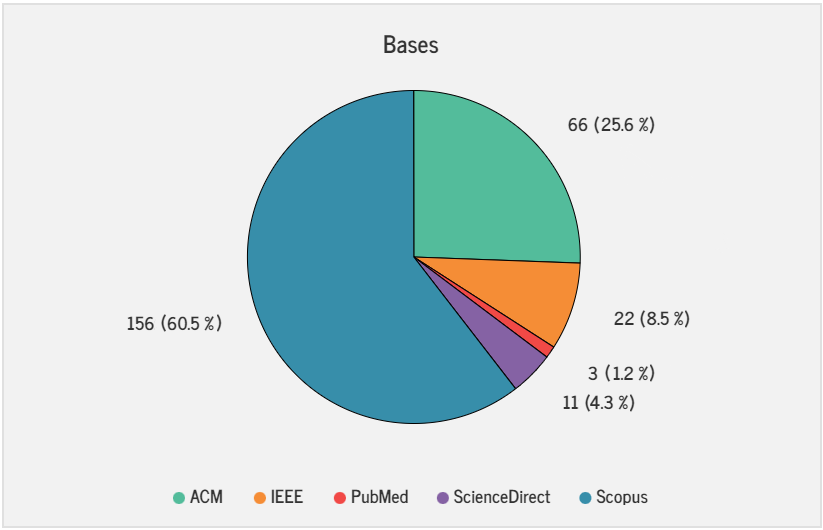
\includegraphics[scale=0.7]{Imagens/msl/artigos_encontrados.png}
	\end{center}
	\legend{Fonte: Autor}
\end{figure}

\subsection{Critérios de Inclusão e Exclusão}

Critérios de inclusão e exclusão foram definidos visando a coerência dos artigos selecionados com o tema deste trabalho, bem como a remoção de artigos incompletos ou indisponíveis.
Os critérios são:

\textbf{Critérios de Inclusão}
\begin{itemize}
  \item O artigo deve propor método, técnica ou padrão para o desenvolvimento de aplicações móveis com acessibilidade para deficientes visuais;
  \item O artigo deve estar disponível na \emph{web};
  \item O artigo deve apresentar texto completo em formato eletrônico;
  \item O artigo deve estar escrito em português ou inglês.
\end{itemize}

\textbf{Critérios de Exclusão}
\begin{itemize}
  \item O artigo não apresenta proposta de aplicação móvel como solução;
  \item O artigo não apresenta aplicativo desenvolvido no contexto do tema deste trabalho;
  \item O artigo é um livro ou parte de um;
  \item O artigo foi publicado antes de 2016;
  \item O artigo está incompleto, indisponível ou duplicado.
\end{itemize}

No processo de seleção dos estudos, inicialmente, foi aplicado o critério de exclusão de artigos duplicados e, em seguida, o de artigos publicados antes de 2016, rejeitando 48 e 65 artigos, respectivamente.
Esses critérios foram priorizados por não haver a necessidade da leitura dos títulos e resumos dos artigos para serem aplicados.
Por fim, após a leitura dos títulos e resumos, mais 112 artigos foram rejeitados, totalizando 225 artigos.
Assim, sendo aceitos 33 artigos para leitura completa e análise.
A \autoref{fig_res_sel} apresenta o resultado dessa seleção.

\begin{figure}[htb]
	\caption{\label{fig_res_sel}Quantidade de artigos aceitos, rejeitados e duplicados na seleção.}
	\begin{center}
	    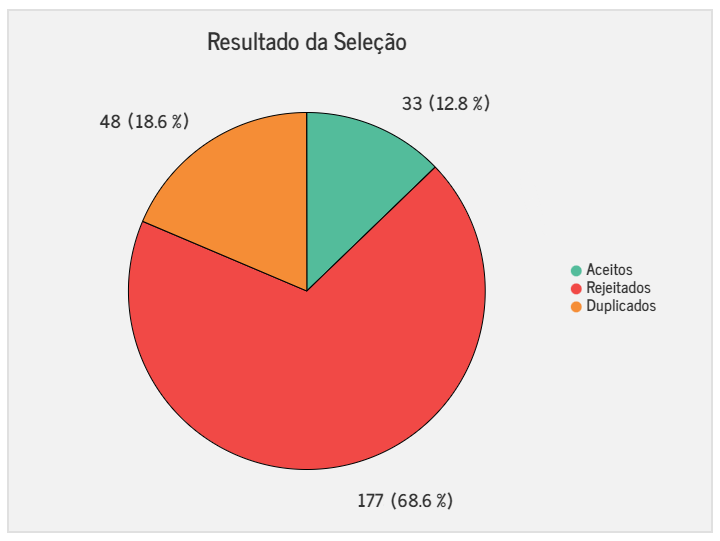
\includegraphics[scale=0.7]{Imagens/msl/resultado_selecao.png}
	\end{center}
	\legend{Fonte: Autor}
\end{figure}

A \autoref{fig_res_sel_base} mostra o resultado da seleção para cada base de busca.
Não houve priorização de bases ao rejeitar artigos duplicados, visto que a ferramenta utilizada possui uma funcionalidade que indica esses artigos, sendo necessário apenas a confirmação.
Com isso, algumas bases como a \emph{PubMed}, cujo resultado da busca retornou apenas 3 artigos sendo 1 duplicado, acabou apresentando poucos ou nenhum artigo aceito.

\begin{figure}[htb]
	\caption{\label{fig_res_sel_base}Quantidade de artigos aceitos e rejeitados por base.}
	\begin{center}
	    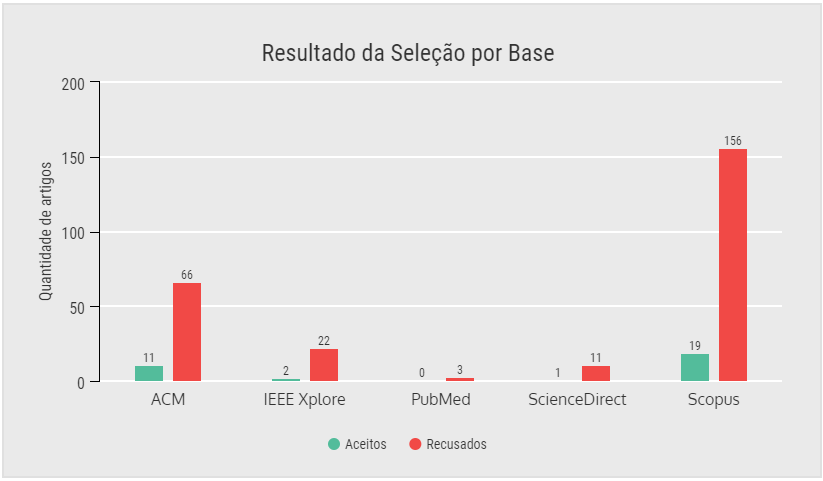
\includegraphics[scale=0.6]{Imagens/msl/resultado_selecao_base.png}
	\end{center}
	\legend{Fonte: Autor}
\end{figure}

\newpage

A frequência dos artigos rejeitados, de acordo com os critérios de exclusão, sendo que, para rejeição, o artigo deveria atender a pelo menos um desses critérios, pode ser observada no gráfico da \autoref{fig_art_rej}, onde é listada para cada critério.

\begin{figure}[htb]
	\caption{\label{fig_art_rej}Quantidade de artigos rejeitados por critério de exclusão.}
	\begin{center}
	    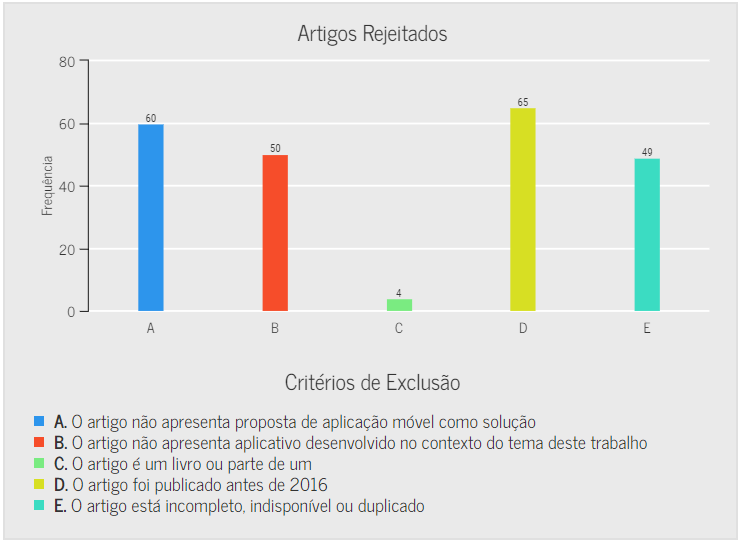
\includegraphics[scale=0.6]{Imagens/msl/artigos_rejeitados.png}
	\end{center}
	\legend{Fonte: Autor}
\end{figure}

Os critérios de exclusão levaram em consideração, principalmente, aspectos como divergência com o tema deste trabalho e não apresentação de aplicação desenvolvida para dispositivos móveis.
Os critérios D e E aparecem com grande frequência na \autoref{fig_art_rej}, valendo ressaltar a ordem na avaliação dos critérios (E, D, A, B e C), onde os artigos que se enquadraram em um dos critérios foram rejeitados, não sendo considerados para avaliação nos demais.
É comum que o critério D seja utilizado no próprio processo de busca dos artigos, filtrando apenas os anos de interesse, porém, como não foi possível adicionar esse filtro às \emph{strings} de busca para todas as bases, foi optado por não utiliza-lo, para manter a consistência nos resultados das buscas.

Após a aplicação dos critérios de exclusão, através da leitura e análise dos títulos e resumos, os artigos restantes, a priori, mostraram se enquadrar em todos os critérios de inclusão.
Assim, a \autoref{fig_art_act_ano} exibe a distribuição desses artigos por ano de publicação e base de busca, mostrando uma clara tendência de alta anual, nos últimos 5 anos, na quantidade de artigos que abordam o tema deste trabalho.
A base \emph{PubMed} foi desconsiderada nessa figura, visto que nenhum artigo dela foi selecionado como mostrou a \autoref{fig_art_rej}.


\begin{figure}[htb]
	\caption{\label{fig_art_act_ano}Quantidade de artigos aceitos por ano e base.}
	\begin{center}
	    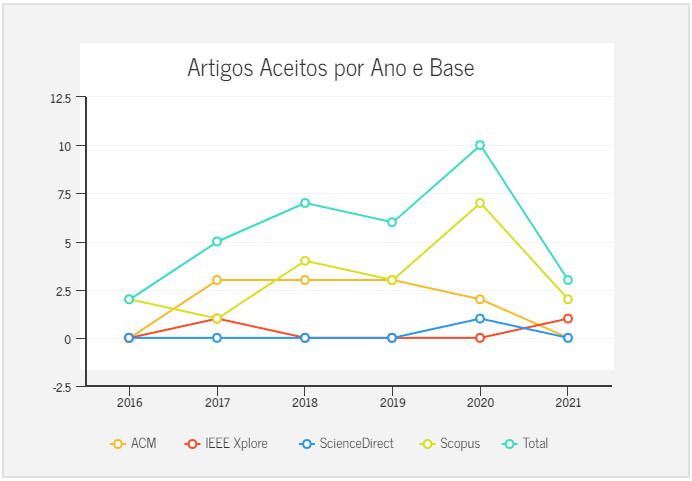
\includegraphics[scale=0.85]{Imagens/msl/artigos_aceitos_ano_base.png}
	\end{center}
	\legend{Fonte: Autor}
\end{figure}

\newpage{}

\subsection{Fase de Extração}

Durante a fase de extração, uma análise mais aprofundada dos artigos foi realizada, inicialmente com intuito de reaplicar os critérios já definidos e utilizados na fase anterior.
O resultado dessa última filtragem pode ser visto na \autoref{fig_fas_ext}.

\begin{figure}[htb]
	\caption{\label{fig_fas_ext}Artigos aceitos e rejeitados na fase de extração.}
	\begin{center}
	    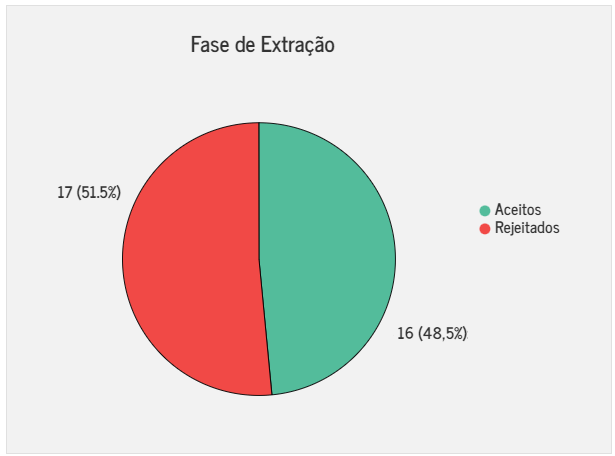
\includegraphics[scale=0.85]{Imagens/msl/fase_extracao_artigos.png}
	\end{center}
	\legend{Fonte: Autor}
\end{figure}

Como a aplicação inicial dos critérios foi realizada com base apenas na leitura dos títulos e resumos dos estudos, não foi possível garantir que os artigos aceitos realmente não se enquadravam nos critérios de exclusão.
Assim, com a análise mais aprofundada e leitura completa dos textos, foi possível identificar 18 artigos que se enquadravam em algum desses critérios, como mostrou a \autoref{fig_fas_ext}.

\newpage

A \autoref{fig_art_rej_fas_ext} mostra a frequência de artigos que foram rejeitados por cada critério de exclusão.
Apenas os critérios com frequência maior que 0 foram considerados na figura.
O principal motivo para rejeição foi o B, onde os trabalhos apresentavam aplicações móveis que não haviam sido desenvolvidas com foco na acessibilidade da aplicação em si.
O segundo foi o A, onde os estudos não apresentavam uma aplicação móvel com acessibilidade à PDV como solução.

\begin{figure}[htb]
	\caption{\label{fig_art_rej_fas_ext}Artigos rejeitados na fase de extração por critério exclusão.}
	\begin{center}
	    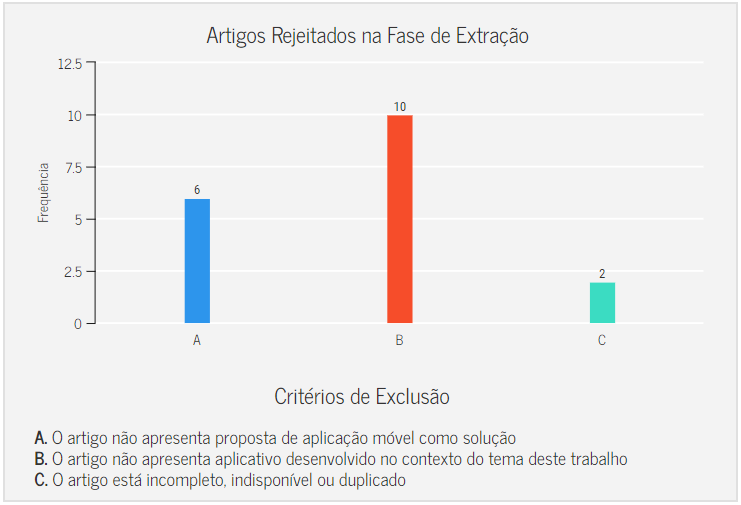
\includegraphics[scale=0.7]{Imagens/msl/artigos_rejeitados_fase_extracao.png}
	\end{center}
	\legend{Fonte: Autor}
\end{figure}

Os 15 estudos aceitos na fase de extração foram reunidos no \autoref{qua-art-ext} com a listagem de informações como o título do estudo, referência e o nome da base de dados em que o artigo foi encontrado.

\begin{quadro}[htb!]
\caption{\label{qua-art-ext}Artigos aceitos na fase de extração.}
\begin{tabular}{|m{1.0cm} | m{8.1cm} | m{2.6cm} | m{2.5cm}|}
  %\hline
    \hline
    \textbf{Sigla} &\textbf{Título} & \textbf{Referência} & \textbf{Base de dados} \\ \hline
    AM1 & \emph{A Mobile Educational Game Accessible to All, Including Screen Reading Users on a Touch-Screen Device} & \cite{Leporini2017} & \emph{ACM Digital Library} \\ \hline
    AM2 & \emph{A model-driven approach to cross-platform development of accessible business apps} & \cite{Christoph2020} & \emph{ACM Digital Library} \\ \hline
    AM3 & \emph{An Accessible Roller Coaster Simulator for Touchscreen Devices: An Educational Game for the Visually Impaired} & \cite{Biase2018} & \emph{IEEE Xplore} \\ \hline
    AM4 & \emph{Application for the Configuration and Adaptation of the Android Operating System for the Visually Impaired} & \cite{Oliveira2018} & \emph{ACM Digital Library} \\ \hline
    AM5 & \emph{Blind and visually impaired user interface to solve accessibility problems} & \cite{Shera2021285} & \emph{Scopus} \\ \hline
    AM6 & \emph{Design and development of a mobile app of drug information for people with visual impairment} & \cite{Amariles2020} & \emph{ScienceDirect} \\ \hline
    AM7 & \emph{Designing multimodal mobile interaction for a text messaging application for visually impaired users} & \cite{Duarte2017} & \emph{Scopus} \\ \hline
    AM8 & \emph{Do You like My Outfit? Cromnia, a Mobile Assistant for Blind Users} & \cite{Giuliana2018} & \emph{ACM Digital Library} \\ \hline
    AM9 & \emph{Improved and Accessible E-Book Reader Application for Visually Impaired People} & \cite{Heesook2017} & \emph{ACM Digital Library} \\ \hline
    AM10 & \emph{MathMelodies 2: A Mobile Assistive Application for People with Visual Impairments Developed with React Native} & \cite{Ducci2018} & \emph{ACM Digital Library} \\ \hline
    AM11 & \emph{Object Recognition and Hearing Assistive Technology Mobile Application Using Convolutional Neural Network} & \cite{Caballero2020} & \emph{ACM Digital Library} \\ \hline
    AM12 & \emph{QUIMIVOX MOBILE 2.0: Application for Helping Visually Impaired People in Learning Periodic Table and Electron Configuration} & \cite{Oliveira2019} & \emph{ACM Digital Library} \\ \hline
    AM13 & \emph{``Talkin' about the weather'': Incorporating TalkBack functionality and sonifications for accessible app design} & \cite{Tomlinson2016377} & \emph{Scopus} \\ \hline
    AM14 & \emph{Users’ perception on usability aspects of a braille learning mobile application ‘mBRAILLE’} & \cite{Nahar2019100} & \emph{Scopus} \\ \hline
    AM15 & \emph{WordMelodies: Supporting Children with Visual Impairment in Learning Literacy} & \cite{Mascetti2019} & \emph{ACM Digital Library} \\ \hline
   % \hline
\end{tabular}
\legend{Fonte: Autor}
\end{quadro}
% !TeX root = ..\Modelo-TCC-DCOMP.tex
\newpage{}

\section{Resultados Encontrados}

Nesta seção, são apresentados os resumos com as principais características, relacionadas ao tema deste trabalho, dos artigos selecionados na fase de extração, visando encontrar respostas para as questões levantadas na definição do protocolo de MSL\@.

\subsection{\emph{A Mobile Educational Game Accessible to All, Including Screen Reading Users on a Touch-Screen Device}}

O estudo realizado por \citeonline{Leporini2017} teve o objetivo levantar informações e possíveis soluções para as dificuldades levantadas por um grupo composto por 6 pessoas cegas ao responder questões de tarefas interativas.
E investigou, através de tarefas interativas como exercícios e questionários, a acessibilidade e usabilidade de gestos e leitores de tela em dispositivos móveis com \emph{touch-screen}.

No artigo é apresentado um \emph{game} que envolveu duas pessoas cegas com experiência na utilização de \emph{smartphones} na fase inicial do planejamento do protótipo.
O jogo funciona como se fosse um ``sistema solar'' com oito planetas, onde cada planeta representa um conjunto de questões e exercícios.
O jogador recebe determinada pontuação cada vez que joga de acordo com os acertos e erros.
As principais funcionalidades do \emph{app} relativas à acessibilidade identificadas foram:

\begin{enumerate}
    \item Contraste de cor para garantir diferentes níveis de acessibilidade;
    \item Apresentações de conteúdos de forma auditiva e visual;
    \item Interação via gestos ou toques;
    \item Suporte auditivo com descrições dos elementos.
\end{enumerate}

Através da avaliação desse protótipo, por cegos, o estudo investigou o suporte de acessibilidade \emph{mobile} multiplataforma do conjunto de especificações técnicas, \emph{WAI-Aria}\footnote{\url{https://www.w3.org/WAI/standards-guidelines/aria/}}, observando problemas na detecção de elementos, devido às suas posições na tela e conteúdos difíceis de identificar na interação com leitores de tela.
Notando também que houve alguma dificuldade por conta de gestos implementados no \emph{app} diferirem dos habituais utilizados pelos usuários no \emph{VoiceOver} do \emph{iOS}.

Apesar dos problemas encontrados, o artigo aponta que o \emph{feedback} foi positivo e os resultados mostraram que os exercícios puderam ser realizados facilmente, por pessoas cegas, através de simples gestos com auxilio dos leitores de tela.

\textbf{Tecnologia utilizada para desenvolvimento:} \emph{Cordova Framework}.

\textbf{Plataforma alvo do \emph{app} desenvolvido:} multiplataforma (\emph{Android} e \emph{iOS}).

\textbf{Público alvo da aplicação:} PDV\@.

\subsection{\emph{A Model-Driven Approach to Cross-Platform Development of Accessible Business Apps}}

Um procedimento comum no processo de desenvolvimento de \emph{software} é considerar a acessibilidade para PDV apenas na etapa final.
Além disso, muitos desenvolvedores não estão cientes de técnicas de software para atender esse grupo, pois o domínio de apps móveis multiplataforma tem recebido uma atenção limitada por pesquisadores.
Foi nesse sentido, que o estudo de \citeonline{Christoph2020} buscou identificar desafios, requisitos e soluções técnicas de acessibilidade, selecionando 28 requisitos a respeito de acessibilidade para aplicações móveis através de uma RSL\@.

O artigo apresenta uma abordagem orientada a modelos que integra conceitos de acessibilidade no desenvolvimento de aplicações móveis multiplataforma em conjunto com protótipos acessíveis à PDV, construídos com base nessa abordagem.
Uma aplicação com foco nos cidadãos que desejam obter informações sobre chuvas fortes e inundações foi desenvolvida, nela os usuários podem ter uma visão de eventos de inundações próximos e compartilhar novos incidentes.

O estudo comparou uma versão da aplicação desenvolvida nativamente que necessitou de 3,400 linhas de código \emph{Java} e 3,200 linhas de código \emph{XML} (gerado de forma semiautomática) com outra versão, com um conjunto similar de funcionalidades.
A nova versão do \emph{app} consistiu em 445 linhas de código \emph{MD²}, \emph{framework} baseado na abordagem orientada a modelos para desenvolvimento móvel multiplataforma através da linguagem de alto nível \emph{Xtend}\footnote{\url{https://www.eclipse.org/xtend/}}.
Principais funcionalidades sobre acessibilidade identificadas:

\begin{enumerate}
    \item Adaptação da \emph{interface} de acordo com as necessidades do usuário;
    \item Integração com os leitores de tela através do fornecimento de descrições em texto para elementos não textuais;
    \item Personalização do contorno de foco do \emph{TalkBack}.
\end{enumerate}

Segundo o artigo, o estudo de caso mostrou que \emph{apps} acessíveis podem ser gerados a partir do modelo de alto nível \emph{MD²}, implementando as técnicas de integração adequadas em cada ponto.
Embora o autor afirme isso, o estudo também deixa claro que ainda havia uma pendência de validação centrada no usuário, visto que o trabalho não implementou todas as técnicas e a solução proposta não foi testada com PDV\@.

\textbf{Tecnologia utilizada para desenvolvimento:} \emph{Xtend, Java} e \emph{Eclipse}.

\textbf{Plataforma alvo do \emph{app} desenvolvido:} multiplataforma (\emph{Android} e \emph{iOS}).

\textbf{Público alvo da aplicação:} PDV interessadas em saber sobre eventos climáticos locais como chuvas fortes e inundações.

\subsection{\emph{An Accessible Roller Coaster Simulator for Touchscreen Devices: An Educational Game for the Visually Impaired}}

O trabalho de \citeonline{Biase2018} apresenta um \emph{app} simulador de montanha russa, baseado em simuladores educacionais já existentes e adaptado para \emph{smartphones}, para ser utilizado em disciplinas Educação Física por pessoas com e sem DV\@.
A aplicação foi desenvolvida para auxiliar no estudo de Energia Mecânica e trás as interações por áudio e tátil como alternativas à visual.
As principais funcionalidades sobre acessibilidade identificadas no \emph{app} foram:

\begin{enumerate}
    \item Os elementos visuais possuem descrições textuais para integração com leitores de tela;
    \item \emph{Feedback} através de ``texto para voz'' (TTS, do inglês \emph{text-to-speech}) e vibração ao clicar em determinados elementos na tela, mesmo com o modo de acessibilidade desativado;
    \item Efeitos sonoros característicos que ilustram os resultados da simulação ao longo do percurso.
\end{enumerate}

Com taxas de 73\% eficácia, 77\% de eficiência e 66\% satisfação do usuário com relação a aplicação desenvolvida, os testes de usabilidade demonstraram que as estratégias de interação propostas são viáveis, com grande potencial para serem utilizadas em propósitos educacionais.

Alguns problemas de acessibilidade afetaram a taxa de satisfação dos usuários, a mantendo em 66\%, tais como dificuldades em seguir a trilha da montanha com apenas um dedo, não ser possível detectar quando o carro está voltando no trilho e falha no comando que altera o foco dos elementos, alterando para o elemento errado.

\textbf{Tecnologia utilizada para desenvolvimento:} \emph{Unity 3D engine}.

\textbf{Plataforma alvo do \emph{app} desenvolvido:} \emph{Android}.

\textbf{Público alvo da aplicação:} Pessoas com e sem DV\@.

\subsection{\emph{Application for the Configuration and Adaptation of the Android Operating System for the Visually Impaired}}

Apesar das vantagens dos dispositivos móveis, alguns desafios da interação de PDV com os sistemas operacionais (SOs) desses dispositivos precisam ser superados, para que a tecnologia alcance um número significativo nesse grupo.
Assim, o estudo de \citeonline{Oliveira2018} visou planejar e desenvolver uma aplicação que automatize as configurações do SO \emph{Android} de acordo com as preferências de acessibilidade de cada PDV, através de comandos de voz.
O artigo apresenta algumas funcionalidades e técnicas relacionadas a acessibilidade que são listadas a seguir:

\begin{enumerate}
    \item Escala de Usabilidade do Sistema (SUS, do inglês \emph{System Usability Scale}) para avaliação de usabilidade da aplicação;
    \item \emph{SpeechRecognizer} do \emph{Android} para reconhecimento de voz;
    \item Eurísticas de Usabilidade de Nielsen (do inglês, \emph{Nielsen Usability Heuristics}) para evitar problemas de acessibilidade já mapeados.
\end{enumerate}

Um protótipo foi desenvolvido e mostrou potencial para ser utilizado como ferramenta para PDV, trazendo benefícios com a possibilidade do uso de comando de voz.
Os testes foram realizados com seis voluntárias com DV, sendo duas parcial e quatro total.
Onde três delas já possuíam experiência com comandos de voz e apenas duas das seis pessoas já haviam realizado a configuração do dispositivo alguma vez.

As voluntárias expressaram avaliações positivas quanto a autonomia, satisfação e usabilidade da aplicação.
E o tempo gasto para realizar as configurações de acessibilidade foi mais curto no \emph{app} desenvolvido que na aplicação padrão do \emph{Android}.

\textbf{Tecnologia utilizada para desenvolvimento:} \emph{Android Studio 2.0}.

\textbf{Plataforma alvo do \emph{app} desenvolvido:} \emph{Android}.

\textbf{Público alvo da aplicação:} PDV\@.

\subsection{\emph{Blind and visually impaired user interface to solve accessibility problems}}

Este estudo realizou uma RSL e testes em várias aplicações móveis para PDV, e dividiu os problemas encontrados em três categorias: organização, apresentação e comportamento (OAC).
Uma aplicação móvel, chamada ``\emph{Read Master}'', também foi desenvolvida no trabalho de \citeonline{Shera2021285}, incorporando soluções para os principais problemas de OAC\@.

\begin{table}[htb]
    \begin{center}
        \ABNTEXfontereduzida
        \caption{Categorias dos problemas identificados.}
        \label{tab-cat-pro-enc-ar5}
        \begin{tabular}{p{2.0cm}|p{5.0cm}}
            %\hline
            \textbf{Código} & \textbf{Categoria} \\
            \hline
            CRR1            & Apresentação       \\
            \hline
            CRR2            & Comportamento      \\
            \hline
            CRR3            & Organizacional     \\
            % \hline
        \end{tabular}
        \legend{Fonte: \citeonline{Siebra2016}}
    \end{center}
\end{table}

Na tabela \autoref{tab-pro-enc-ar5} estão listados os problemas identificados pelo estudo.
Os códigos na coluna ``Categoria'' se referem as categorias da \autoref{tab-cat-pro-enc-ar5}.

\begin{table}[htb]
    \begin{center}
        \ABNTEXfontereduzida
        \caption{Problemas de acessibilidade encontrados por categoria.}
        \label{tab-pro-enc-ar5}
        \begin{tabular}{p{1.2cm}|p{11.5cm}|p{1.5cm}}
            %\hline
            \textbf{Código} & \textbf{Problema}                                                                                 & \textbf{Categoria} \\
            \hline
            AM11            & Falta de consistência no \emph{layout} e terminologias                                            & CRR1               \\
            \hline
            AM12            & Leitor de tela fornecendo \emph{feedbacks} confusos                                               & CRR1               \\
            \hline
            AM13            & Leitor de tela quebrando                                                                          & CRR2               \\
            \hline
            AM14            & Ouvir cabeçalhos e títulos das páginas de forma redundante antes de detectar o conteúdo das telas & CRR2               \\
            \hline
            AM15            & Conteúdos na tela da aplicação móvel                                                              & CRR3               \\
            \hline
            AM16            & Fluxo de tarefas                                                                                  & CRR3               \\
            \hline
            AM17            & Não entendimento da sequência natural de leitura                                                  & CRR3               \\
            \hline
            AM18            & Não entendimento do fluxo natural de tarefas                                                      & CRR3               \\
            \hline
            AM19            & Problemas de navegação                                                                            & CRR3               \\
            \hline
            AM110           & Sobrecarga de informações                                                                         & CRR3               \\
            % \hline
        \end{tabular}
        \legend{Fonte: \citeonline{Shera2021285}}
    \end{center}
\end{table}

O \emph{app} desenvolvido consistiu em duas funcionalidades principais: fornecer informações cientificas e \emph{quizzes} de múltipla escolha.
As principais técnicas e funcionalidades identificadas no estudo para o suporte de acessibilidade foram:

\begin{enumerate}
    \item \emph{SUS} para avaliação de usabilidade da aplicação;
    \item Leitor de tela embutido através de TTS\@.
    \item Levantamento e categorização dos principais problemas de acessibilidade em \emph{apps} móveis.
\end{enumerate}

Uma avaliação de usabilidade do \emph{app}, com 56 PDV, foi conduzida e validada com foco na experiência de usuários com DV\@.
Os resultados mostraram que a organização da aplicação estava 100\% efetiva tanto para usuários os cegos quanto para os com DV parcial.
Já quanto a eficiência, a dos usuários com DV parcial se mostrou maior que a dos cegos.
O nível mais alto de satisfação, quanto as 3 categorias de problemas avaliados, para usuários com DV total, estava na apresentação com 87,62\%, enquanto para os com visão parcial estava tanto na organização quanto na apresentação com 89,21\%.
No geral, o estudo indica que a aplicação reduziu a gravidade dos problemas de OPB, oferecendo alta usabilidade.

\textbf{Tecnologia utilizada para desenvolvimento:} Não informado.

\textbf{Plataforma alvo do \emph{app} desenvolvido:} \emph{Android}.

\textbf{Público alvo da aplicação:} PDV\@.

\subsection{\emph{Design and development of a mobile app of drug information for people with visual impairment}}

Esse trabalho foi desenvolvido na Colombia, onde a falta de acesso à informações acessíveis
de rótulos de medicamentos como contraindicações, armazenamento, data de validade e dosagem foi identificada como uma
das principais barreiras no uso de medicamentos por PDV \cite{Amariles2020}.

Nesse contexto, uma aplicação \emph{mobile}, chamada \emph{FarmaceuticApp}, foi desenvolvida no estudo.
A principal funcionalidade do \emph{app} é a de buscar por informações de medicamentos, onde essas informações são apresentadas ao usuário de forma acessível e a busca pode ser realizada por vários meios, esses que serão listados adiante.

As principais técnicas e funcionalidades identificadas, relacionadas à acessibilidade e utilizadas no desenvolvimento dessa solução, foram:

\begin{enumerate}
    \item Tamanho da fonte das letras personalizável;
    \item Vibração e sons para alertar o usuário do resultado da busca;
    \item \emph{Tutorial} com possibilidade de ser visto novamente;
    \item Possibilidade de busca por \emph{barcode} e \emph{qrcode}, foto, comando de voz e texto;
    \item Possibilidade de ativar e desativar o assistente de voz do \emph{app}.
\end{enumerate}

\textbf{Tecnologia utilizada no desenvolvimento:} \emph{Java, Android Studio, Accessibility Scanner App}, e o \emph{Test Lab do Firebase}.

\textbf{Plataforma alvo do \emph{app} desenvolvido:} \emph{Android}.

\textbf{Público alvo da aplicação:} PDV que buscam obter informações de rótulos de medicamentos\@.

O estudo envolveu 48 PDV, das quais 69\% necessitavam de assistência para o uso de medicamentos e 90\% possuíam celulares, sendo 93\%  deles com o SO \emph{Android}.
Na avaliação final, 100\% dos usuários disseram utilizariam o \emph{app} e o avaliaram entre 4 e 5 estrelas (bom e muito bom).


\subsection{\emph{Designing multimodal mobile interaction for a text messaging application for visually impaired users}}

Apesar da inclusão de opções de acessibilidade, os SOs móveis ainda enfrentam uma falta de suporte adequado para alguns tipos de atividades e contextos, como é o exemplo da escrita de textos para PDV, uma tarefa que acaba consumindo muito tempo.
Além disso, os usuários geralmente necessitam utilizar as duas mãos para escrever mensagens, o que mostra ser um problema para cegos que necessitam carregar bengala ou possuem cão guia, assim restando apenas uma mão livre.

Nesse contexto, a abordagem proposta no estudo de \citeonline{Duarte2017}, através do protótipo de um \emph{app} para envio de mensagens, visou uma interação com o \emph{smartphone} com as mãos livres, através de técnicas multimodais, especialmente o uso de gestos em combinação com comandos de voz.

Os gestos são utilizados como gatilhos para ações.
Assim, quando um gesto é reconhecido, ele ativa alguma função, que geralmente ativa o ``reconhecedor de fala'' ou o TTS\@.
Por exemplo, existe um gesto para a ação de adicionar uma nova mensagem, ao reconhece-lo, o \emph{app} ativa o reconhecedor de fala para que o usuário dite o que deve ser escrito na mensagem.
Um outro gesto ativa a função para revisão da mensagem escrita, ao ser reconhecido, o TTS é ativado e a mensagem é lida palavra a palavra.
As principais características relacionadas à acessibilidade identificadas nessa solução foram:

\begin{enumerate}
    \item Reconhecimento de voz;
    \item Reconhecimento de gestos;
    \item Sintese de fala.
    \item Possibilidade de revisar as mensagens escritas de maneira acessível;
    \item Possibilidade de parar a narração durante a revisão da mensagem e editar palavras especificas;
    \item Aplicação de questionário da Escala de Usabilidade do Sistema, SUS\@.
\end{enumerate}

\textbf{Tecnologia utilizada no desenvolvimento:} \emph{Java, Android Studio, Accessibility Scanner App}, e o \emph{Test Lab do Firebase}.

\textbf{Plataforma alvo do \emph{app} desenvolvido:} \emph{Android}.

\textbf{Público alvo da aplicação:} PDV\@.

Uma pesquisa foi realizada com 9 usuários com DV e resultou em \emph{feedbacks} positivos, principalmente a respeito da interação por gestos.
Na avaliação da usabilidade das aplicações, através da escala SUS, ambas atingiram 74 pontos, considerada uma alta pontuação.

O estudo também trouxe comparativo de performance dos usuários na realização de tarefas no \emph{app} de envio de mensagem padrão com o \emph{app} desenvolvido.
Os resultados mostraram que na realização de tarefas fáceis, a performance do \emph{app} era pouco superior a alternativa padrão do sistema.
Porém, passa-se a notar grandes diferenças a favor do \emph{app} desenvolvido em tarefas consideradas normais e difíceis, com cerca de 30\% e 50\% mais performance, respectivamente, para a solução desenvolvida em relação ao \emph{app} padrão.

\subsection{\emph{Do You like My Outfit? Cromnia, a Mobile Assistant for Blind Users}}

O objetivo do estudo de \citeonline{Giuliana2018} foi projetar uma solução assistiva que pudesse prover autonomia à pessoas cegas em suas atividades diárias.
Especialistas na área de deficiência visual, de clínicos à profissionais de reabilitação vocacional e operadores do campo de cuidados sociais, participaram do estudo.

%Uma pesquisa, em forma de questionário, com 10 pessoas foi realizada como parte de um projeto europeu que visa definir um roteiro de compras inovador para PDV\@.

O processo de análise e projeto envolveu, desde o início, a participação de 4 pessoas cegas da \emph{Italian Blind Union}, que se voluntariaram para colaborar com a equipe de \emph{design} de usabilidade.
Entre as tarefas diárias que mais se esperava autonomia a de se vestir com uma combinação de cores e roupas adequadas se mostrou ser o maior interesse para as PDV, essas que geralmente dependem de ajudantes para isso.
Assim, uma aplicação \emph{mobile} foi projetada, visando a autonomia de PDV, total ou parcial, nesse ato cotidiano de se vestir.

\begin{enumerate}
    \item Integração com leitores de tela;
    \item Tamanho de fontes e \emph{labels} adaptáveis de acordo com o tipo de deficiência;
    \item Sistema de notificações simples e imediato;
    \item Resposta em tempo real.
\end{enumerate}

\textbf{Tecnologia utilizada no desenvolvimento:} Não informado.

\textbf{Plataforma alvo do \emph{app} desenvolvido:} \emph{iOS}.

\textbf{Público alvo da aplicação:} PDV\@.

Como resultado do estudo uma aplicação chamada de \emph{Cromnia}, que possibilita que os usuários reconheçam cores, padrões e combinações de cores, considerando a iluminação do ambiente foi desenvolvida.
O \emph{app} é bem simples e consiste em uma única \emph{interface}, parecida com a padrão da câmera do sistema \emph{iOS}.
O estudo levantou que já existiam soluções no mercado para esse problema, porém a ideia de uma ferramenta paga não foi bem aceita pelos entrevistados, que observaram que muitos nem poderiam pagar.

Os testes envolveram 6 PDV com parcial e 6 com DV total.
Os participantes gostaram dos benefícios do \emph{app} e se mostraram ansiosos para experimentar novas versões, pensando em quando poderão utilizar o aplicativo de fato no dia-a-dia.
O \emph{app} está disponível na \emph{AppStore} e conta com alto número de \emph{downloads}.

\subsection{\emph{Improved and Accessible E-Book Reader Application for Visually Impaired People}}

Embora livros digitais já estejam estabelecidos internacionalmente, não são satisfatórios em termos de acessibilidade e \emph{interface}.
Por conta disso, o estudo de \citeonline{Heesook2017} apresenta um aplicativo leitor de \emph{e-book} acessível à PDV, que tem o objetivo de suprimir limitações como falta de novos livros, ausência de textos alternativos e navegação desconfortável dos atuais formatos acessíveis, em áudio e \emph{Braille}.

Um levantamento de requisitos de usuário foi realizado através de questionário e cerca 70\% dos requisitos foram implementados.
O \emph{app} possibilita a realização de busca, \emph{download} e leitura de conteúdos no formato \emph{EPUB3} e possui controles para inciar, parar, avançar e retroceder a leitura.
Quanto à acessibilidade, foram identificadas as seguintes soluções:

\begin{enumerate}
    \item Suporte para comandos de voz;
    \item Configurações de alto contraste;
    \item Sintese de voz para leitura dos \emph{e-books};
    \item Tamanho dos botões e espaçamentos adequados à PDV\@.
\end{enumerate}

\textbf{Tecnologia utilizada no desenvolvimento:} Não informado.

\textbf{Plataforma alvo do \emph{app} desenvolvido:} \emph{iOS}.

\textbf{Público alvo da aplicação:} PDV que gostam de livros\@.

Nos resultados dos testes, realizados com 12 PDV (7 experientes e 5 sem experiência), o estudo mostrou que a média de satisfação dos usuários foi de aproximadamente 75\% nos testes de usabilidade, realizados em 3 fases, com usuários com e sem experiência.
Onde tempo médio de execução das tarefas foi de 92 segundos para usuários não experientes e 82 segundos para experientes.
Usuários experientes enfrentaram erros relacionados a \emph{login}, configuração e busca por tentarem utilizar suas próprias abordagens baseadas em outras aplicações.

\subsection{\emph{MathMelodies 2: A Mobile Assistive Application for People with Visual Impairments Developed with React Native}}

Esse artigo apresenta a experiência do desenvolvimento do \emph{MathMelodies 2}, uma aplicação para ajudar crianças de 1 a 5 anos com DV no estudo de matemática.
A aplicação apresenta 13 tipos de exercícios e diferentes níveis de dificuldade.
Esses exercícios se passam dentro de contos de fantasia, onde a criança tem que resolvê-los para avançar na história.

A primeira versão foi desenvolvida em 2013 através de uma campanha de \emph{crowdfunding} e lançada para \emph{iPad} de forma gratuita.
O \emph{design} do novo \emph{app} seguiu princípios que derivados da experiência e do \emph{feedback} dos usuários da versão anterior.
Uma das demandas mais comuns foi a de disponibilização do \emph{app} para outras plataformas, \emph{Android} e \emph{iOS}.
Assim, nesse trabalho, \citeonline{Ducci2018}, desenvolve essa nova versão como um protótipo, utilizando \emph{React Native} para reduzir o esforço de desenvolvimento.
As principais técnicas e funcionalidades para acessibilidade, utilizadas nesse estudo, são listadas a seguir:

\begin{enumerate}
    \item Implementação nativa para \emph{iOS} e \emph{Android} de componentes não acessíveis no \emph{React Native};
    \item Elementos chave de interação sempre posicionados na mesma parte da tela, em locais de fácil acesso;
    \item Tamanho dos ícones e componentes adaptáveis de acordo com tamanho da tela;
    \item Todos os elementos visíveis na tela sem necessidade de rolagem;
    \item Cores de fundo uniformes e neutras;
    \item Interações por gestos simples.
\end{enumerate}

\textbf{Tecnologia utilizada para desenvolvimento:} \emph{React Native}.

\textbf{Plataforma alvo do \emph{app} desenvolvido:} multiplataforma (\emph{Android} e \emph{iOS}).

\textbf{Público alvo da aplicação:} Crianças com DV\@.

Embora as funcionalidades básicas tenham sido contempladas pelo \emph{framework} utilizado, uma funcionalidade avançada que foi requerida não era suportada.
Por conta disso, foi necessário desenvolver componentes adicionais nativamente, isto é, utilizando as tecnologias especificas para cada plataforma.

Testes preliminares, realizados com duas pessoas (uma com DV parcial e outra total), sugeriram que a aplicação estava totalmente acessível.
Assim, o estudo conclui que \emph{React Native} é uma escolha válida para o desenvolvimento de aplicações acessíveis.

\subsection{\emph{Object Recognition and Hearing Assistive Technology Mobile Application Using Convolutional Neural Network}}

A falta de aplicações móveis que atendam pelo menos as necessidades mais comuns de PDV motivou a realização do trabalho de \citeonline{Caballero2020}, que desenvolveu uma aplicação com objetivo de atender as necessidades desse grupo através de tecnologias de Reconhecimento de Objetos (RO) e TTS\@.

O \emph{app} utiliza algoritmos de \emph{Convolutional Neural Network} (CNN), solução de aprendizado de máquina reconhecida como um poderoso método para reconhecimento de imagens, para identificar detalhes em imagens e narra-los para o usuário através do TTS\@.
O artigo se concentra mais na apresentação da API utilizada para o RO, mostrando pouco sobre a aplicação \emph{mobile}, ainda assim, foram identificadas as seguintes características de acessibilidade no \emph{app}:

\begin{enumerate}
    \item Reconhecimento de detalhes de imagens;
    \item Sintese dos resultados do RO por voz.
\end{enumerate}

\textbf{Tecnologia utilizada para desenvolvimento:} Não informado.

\textbf{Plataforma alvo do \emph{app} desenvolvido:} \emph{Android}.

\textbf{Público alvo da aplicação:} PDV\@.

O estudo realizou a revisão de diferentes estudos e tecnologias que utilizam CNN, um dos principais estudos citados foi publicado em 2015 na Conferência Brasileira de Sistemas Inteligentes (BRACIS), este que utiliza RO para um sistema de navegação inteligente que possibilita que robôs interajam e determinem o comportamento de objetos.
Através dos trabalhos relacionados citados, o artigo apresenta o RO sendo utilizado para inclusão social de PDV\@.

Os resultados mostraram que CNN tem potencial para classificar coisas vivas e objetos em ambientes interiores e exteriores com alta precisão, através de imagens públicas que serviram como base para treinamento.
Assim, possibilitando um desempenho funcional e confiável do sistema em beneficio das PDV através do \emph{app} desenvolvido.

\subsection{\emph{QUIMIVOX MOBILE 2.0: Application for Helping Visually Impaired People in Learning Periodic Table and Electron Configuration}}

Muito ainda precisa ser feito quanto a inclusão de PDV no processo de ensino e aprendizagem de química, por requerer de muitos recursos visuais.
E, embora exista uma quantidade significativa de \emph{apps} que auxiliam no ensino de química, os mesmos não são acessíveis aos DV, mesmo com o uso de leitores de tela.

É nesse sentido que o estudo de \citeonline{Oliveira2019} introduziu uma nova versão do \emph{``Quimivox Mobile 2.0''}, aplicativo que apresenta informações acessíveis à DV sobre a tabela periódica e, na nova versão, a configuração eletrônica dos elementos químicos.
A interação do \emph{app} é baseada em gestos e comandos de voz, com as informações sendo apresentadas graficamente e por síntese de voz, através do \emph{TalkBack}.

A aplicação utiliza de técnicas de gestos já utilizadas em outras ferramentas que consistem em deslizar com os dedos em quatro direções.
Esses gestos foram complementados com outros específicos para a realização de ações na aplicação, tais como a ativação do reconhecimento de voz e uma opção para retornar a tela anterior.
Segue abaixo as principais técnicas e funcionalidades para acessibilidade identificadas no estudo:

\begin{enumerate}
    \item Interação por reconhecimento de voz e gestos;
    \item Tamanhos de fontes de letras ampliados;
    \item Alto contraste (fundos pretos e textos brancos);
    \item Possibilidade de escolha de cores do \emph{app} para melhorar a legibilidade para pessoas daltônicas;
    \item \emph{Feedback} sonoro mesmo com \emph{Talkback} desativado.
\end{enumerate}

\textbf{Tecnologia utilizada para desenvolvimento:} \emph{Java, Android Studio} e \emph{API Airy}.

\textbf{Plataforma alvo do \emph{app} desenvolvido:} \emph{Android} 4.0 ou superior.

\textbf{Público alvo da aplicação:} PDV interessadas no aprendizado de Química\@.

Os usuários apontaram o comando de voz como a funcionalidade que mais facilitou na utilização da \emph{app}.
Na avaliação de uma das PDV, participante dos testes, o desenvolvimento de manual poderia contribuir com melhor entendimento do funcionamento do aplicativo.
Outras sugestões foram a ampliação dos tipos de toques na tela e o aumento na velocidade da voz sintetizada.

O artigo conclui que os participantes aprovaram a nova versão, avaliando positivamente o \emph{app}, indicando que a maior dificuldade estava na pouca prática no uso de dispositivos móveis por parte de alguns DV\@.
E relata que essa dificuldade estava relacionada aos gestos, onde a maioria fez algum comentário negativo, citando 5 desses participantes.

Porém, o autor supõe que, com a prática no uso dos gestos, essa dificuldade poderia ser diminuída significativamente, citando o reconhecimento da falta de experiência na utilização de dispositivos móveis por 4 participantes como justificativa, sendo que apenas um deles, chamado P10, fazia parte dos 5 participantes citados pelos comentários negativos.

\subsection{\emph{``Talkin' about the weather'': Incorporating TalkBack functionality and sonifications for accessible app design}}

Informações a respeito do clima atual e previsões são especialmente importantes para PDV, visto que podem afetar suas as decisões do cotidiano, como escolhas de rotas, roupas e tecnologias assistivas que impactam significativamente seu trajeto.
Porém, essas pessoas enfrentam péssimas experiencias tentando buscar informações sobre o clima nos dispositivos móveis, geralmente por conta dos erros entre as informações na tela e a ordem em que os leitores de tela as apresentam, além dos apps serem cheios de imagens e ícones que costumam não apresentar descrição para o usuário a menos que possa enxerga-las.

Assim, \citeonline{Tomlinson2016377}, nesse estudo, projetou um \emph{app} de clima que visa ser acessível à usuários que dependem de leitores de tela.
O estudo realizou uma análise das necessidades dos usuários com DV, levantando quais eram as informações importantes e em qual ordem eles gostariam de consumi-las.
As principais soluções quanto à acessibilidade identificadas foram:

\begin{enumerate}
    \item Alternativa aos ícones padrões utilizados para indicação através dos chamados ``Ícones auditivos'';
    \item Utilização constante do \emph{TalkBack} durante o processo de desenvolvimento;
    \item Interface com alto contraste (textos brancos em fundo preto), visando a experiência de usuário (UX) de PDV\@;
    \item Integração com \emph{Talkback} seguindo as Diretrizes de Acessibilidade do \emph{Google}.
\end{enumerate}

``Ícones auditivos'' emitem sons breves, baseados nos sons reais do cotidiano, e servem alternativa para representação dos ícones visuais de clima, como o ícone de chuva, representado por sons que remetem ao evento.

\textbf{Tecnologia utilizada para desenvolvimento:} Não informado.

\textbf{Plataforma alvo do \emph{app} desenvolvido:} \emph{Android}.

\textbf{Público alvo da aplicação:} PDV que necessitam saber sobre o clima\@.

Nos testes de usabilidade, 7 participantes responderam que utilizaram o \emph{app} por pelo menos seis dias durante a semana e, no geral, reportaram terem obtido experiência tão boa ou melhor que nos \emph{apps} de clima que já utilizaram anteriormente.

\subsection{\emph{Users’ perception on usability aspects of a braille learning mobile application ‘mBRAILLE’}}

Estudantes com DV enfrentam dificuldades ou incapacidade, a depender do nível de DV, para obter informações visuais, o que torna o processo de aprendizagem deles mais difícil que o dos outros.
Nesse artigo, \citeonline{Nahar2019100}, apresenta o \emph{mBRAILLE}, \emph{app} que foi desenvolvido em \emph{Bangladesh} para auxiliar PDV no processo de autoaprendizagem de \emph{Braille}, sem ou com dependência mínima de outras pessoas.
Embora a publicação não apresente muitos detalhes do processo de desenvolvimento, sequer mencionam leitores de tela, algumas características relacionadas à acessibilidade utilizadas na solução foram identificadas, seguem:

\begin{enumerate}
    \item \emph{Tutorial} para auxiliar o usuário na utilização do \emph{app};
    \item \emph{Feedback} por vibração e áudio;
\end{enumerate}

\textbf{Tecnologia utilizada para desenvolvimento:} Não informado.

\textbf{Plataforma alvo do \emph{app} desenvolvido:} \emph{Android}.

\textbf{Público alvo da aplicação:} Estudantes de \emph{Bangladesh} com DV\@.

O estudo avaliou 4 aspectos de usabilidade (aprendizagem, interface e funcionalidades, acessibilidade e auto descritividade) do \emph{app} através de testes com 5 usuários com DV, que realizaram a avaliação após utilizarem a aplicação por 2 semanas, mostrando resultados de avaliação média satisfatórios, de 6 ou acima, numa escala de 0 a 7.

O estudo teve a uma limitação de apenas 5 participantes, sendo todos experientes em \emph{Braille}.
Assim, o artigo menciona que trabalhos futuros concentrar-se-ão em avaliar e testar a efetividade do aprendizado de \emph{Braille} através do \emph{app}, com um grande número de participantes de diferentes escolas.


\subsection{\emph{WordMelodies: Supporting Children with Visual Impairment in Learning Literacy}}

As ferramentas educacionais de escolas primarias frequentemente não são acessíveis para crianças com DV\@.
Além disso, os livros costumam ser ricos em conteúdos gráficos com o intuito de engajar os alunos, impactando na acessibilidade mesmo quando estão disponíveis no formato digital.
Da mesma forma, \emph{apps} educacionais frequentemente possuem conteúdos gráficos interativos de maneira inacessível à PDV\@.

Visando amenizar esses problemas, o artigo de \citeonline{Mascetti2019} apresenta o \emph{WordMelodies}, uma aplicação \emph{mobile} inclusiva e multiplataforma que tem como objetivo ajudar crianças com DV na adquisição de habilidades básicas de literatura com 8 tipos de exercícios.
A aplicação foi projetada e avaliada por 3 especialistas no dominio de tecnologias assistivas e educação para crianças com DV\@.
As principais características relativas à acessibilidade encontradas no artigo foram:

\begin{enumerate}
    \item Elementos chave de interação sempre posicionados na mesma parte da tela, priorizando os cantos da tela;
    \item Interações por gestos como ``arrastar e soltar'' com descrição auditiva;
    \item Descrição alternativa em texto dos elementos de tela para integração com leitores de tela.
\end{enumerate}

\textbf{Tecnologia utilizada para desenvolvimento:} \emph{React Native}.

\textbf{Plataforma alvo do \emph{app} desenvolvido:} multiplataforma (\emph{Android} e \emph{iOS}).

\textbf{Público alvo da aplicação:} Crianças com DV\@.

Na avaliação dos especialistas, o \emph{app} se mostrou totalmente acessível, exceto por um problema que afetou a utilização do usuário ao navegar entre os elementos utilizando leitores de tela.
Nessa navegação, a ordem dos elementos não corresponde com a ordem lógica apresentada na tela, problema que ocorreu por uma limitação do \emph{kit} de ferramentas da plataforma de desenvolvimento utilizada, o \emph{React Native}.

Um dos principais desafios no desenvolvimento foi alcançar uma funcionalidade de ``arrastar e soltar'' acessível e fácil de utilizar.
Pois, no \emph{React Native} esse componente não fornece suporte à acessibilidade, sendo necessário o desenvolvimento de um componente nativo tanto no \emph{iOS} como no \emph{Android}, para prover informações auditivas ao usuário enquanto ele utiliza o componente.

\section{Estudos Relacionados}

Durante o processo de seleção de artigos do MSL, foram encontrados alguns estudos secundários, estudo que realiza uma revisão de estudos primários relacionados a um tema específico \cite{Kitchenham2007}.
Embora tenham sido rejeitados no MSL, por se enquadrarem em algum dos critérios definidos na seção anterior, os estudos que realizaram revisões dentro do tema estudado neste trabalho foram considerados como estudos relacionados.

Assim, esta seção apresenta os principais problemas e propostas de soluções relacionados à acessibilidade de aplicações para dispositivos móveis identificados por esses estudos.
No \autoref{qua-art-rev-sis} estão listadas as informações de cada um desses estudos secundários.

\begin{quadro}[htb!]
  \caption{\label{qua-art-rev-sis}Estudos relacionados identificados no processo de MSL.}
  \begin{tabular}{|m{1.2cm} | m{8.1cm} | m{2.7cm} | m{2.5cm}|}
    %\hline
    \hline
    \textbf{Código} & \textbf{Título}                                                                                                             & \textbf{Referência}  & \textbf{Base de dados}     \\
    \hline
    AR1             & \emph{Accessibility of Mobile Applications: Evaluation by Users with Visual Impairment and by Automated Tools}              & \cite{Mateus2020}    & \emph{ACM Digital Library} \\
    \hline
    AR2             & \emph{Can Everyone use my app? An Empirical Study on Accessibility in Android Apps}                                         & \cite{Vendome201941} & \emph{Scopus}              \\
    \hline
    AR3             & \emph{Effect of UX Design Guideline on the information accessibility for the visually impaired in the mobile health apps}   & \cite{Kim20191103}   & \emph{Scopus}              \\
    \hline
    AR4             & \emph{Mobile Device Accessibility for the Visually Impaired: Problems Mapping and Empirical Study of Touch Screen Gestures} & \cite{Damaceno2016}  & \emph{ACM Digital Library} \\
    \hline
    AR5             & \emph{Observation Based Analysis on the Use of Mobile Applications for Visually Impaired Users}                             & \cite{Siebra2016}    & \emph{ACM Digital Library} \\
    \hline
    AR6             & \emph{Prioritization of mobile accessibility guidelines for visual impaired users}                                          & \cite{Quispe2020}    & \emph{Scopus}              \\
    \hline
    % \hline
  \end{tabular}
  \legend{Fonte: Autor}
\end{quadro}

% ---
\subsection{\emph{Accessibility of Mobile Applications: Evaluation by Users with Visual Impairment and by Automated Tools}}
% ---

O artigo apresenta um estudo comparativo de problemas de acessibilidade encontrados pelas ferramentas automatizadas MATE (\emph{Mobile Accessibility Testing}) e \emph{Accessibility Scanner}, com os problemas encontrados em um estudo anterior envolvendo 11 usuários com DV\@.
Além disso, o trabalho sumarizou e categorizou os problemas mais encontrados pelos usuários.
As principais categorias são listadas na \autoref{tab-cat-pro-1}.

\begin{table}[htb]
  \begin{center}
    \ABNTEXfontereduzida
    \caption{Categorias dos tipos de problemas mais identificados.}
    \label{tab-cat-pro-1}
    \begin{tabular}{p{2.0cm}|p{7cm}}
      %\hline
      \textbf{Código} & \textbf{Categoria}                       \\
      \hline
      CPF1            & Botões                                   \\
      \hline
      CPF2            & Características do Sistema               \\
      \hline
      CPF3            & Conteúdo e Significado                   \\
      \hline
      CPF4            & Controles, formulários e funcionalidades \\
      \hline
      CPF5            & Imagem                                   \\
      % \hline
    \end{tabular}
    \legend{Fonte: \citeonline{Christoph2020}}
  \end{center}
\end{table}

Na \autoref{tab-pro-blind-1} são listados os principais tipos de problemas, que apresentaram um total de pelo menos 10 observações.
As categorias, de acordo com a \autoref{tab-cat-pro-1}, e o número total de observações para cada tipo de DV\@ (total ou parcial) também são relacionados à cada tipo de problema.
Como o artigo só menciona os tipos problemas encontrados com maior frequência por cada tipo de usuário, o número de observações de alguns não estão presentes na \autoref{tab-pro-blind-1}.

\begin{table}[htb]
  \begin{center}
    \ABNTEXfontereduzida
    \caption{Problemas mais frequentes encontrados pelos usuários por tipo de DV.}
    \label{tab-pro-blind-1}
    \begin{tabular}{p{1.2cm}|p{8.7cm}|p{1.4cm}|p{0.6cm}|p{0.6cm}|p{0.7cm}}
      %\hline
      \textbf{Código} & \textbf{Problema}                                                       & \textbf{Categoria} & \textbf{DVT} & \textbf{DVP} & \textbf{Total} \\
      \hline
      AR1P1           & \emph{Feedback} inapropriado                                            & CPF4               & 34           & 15           & 49             \\
      \hline
      AR1P2           & Falta de informações                                                    & CPF1               & 22           & 8            & 30             \\
      \hline
      AR1P3           & Usuários presumiram que era uma funcionalidade                          & CPF4               & 18           & 9            & 27             \\
      \hline
      AR1P4           & Funcionalidades confusas ou não claras                                  & CPF4               & 25           & -            & 25             \\
      \hline
      AR1P5           & Apresentação padrão de elementos de controle ou formulário não adequada & CPF4               & 11           & 12           & 23             \\
      \hline
      AR1P6           & Sequências de interação confusas ou não claras                          & CPF4               & 15           & 6            & 21             \\
      \hline
      AR1P7           & Usuários não entenderam sentido do conteúdo                             & CPF3               & 15           & 5            & 20             \\
      \hline
      AR1P8           & Organização do conteúdo inconsistente                                   & CPF3               & 12           & 6            & 18             \\
      \hline
      AR1P9           & Funcionalidade não funciona como esperado                               & CPF4               & 6            & 10           & 16             \\
      \hline
      AR1P10          & Funcionalidades dos botões confusas ou não claras                       & CPF1               & 15           & -            & 15             \\
      \hline
      AR1P11          & Expectativa de funcionalidade que não existe                            & CPF4               & 10           & 5            & 15             \\
      \hline
      AR1P12          & Sem alternativa textual                                                 & CPF5               & 14           & -            & 14             \\
      \hline
      AR1P13          & Sistema muito lento                                                     & CPF2               & -            & 11           & 11             \\
      \hline
      AR1P14          & Significado no conteúdo está perdido                                    & CPF3               & 6            & 4            & 10             \\
      % \hline
    \end{tabular}
    \legend{Fonte: \citeonline{Christoph2020}}
  \end{center}
\end{table}

Os resultados do estudo mostraram que 36 tipos de problemas foram encontrados somente pelos usuários, 11 somente pelas ferramentas e 3 por ambos os métodos.
Evidenciando assim a necessidade de utilização de mais de um método para identificação dos problemas de acessibilidade.
Além disso, o estudo mostrou a importância da utilização dessas ferramentas automatizadas, visto que parte significativa dos problemas podem ser identificados ainda no processo de desenvolvimento, reduzindo o esforço e, consequentemente, o custo para solucioná-los.

% ---
\subsection{\emph{Can Everyone use my app? An Empirical Study on Accessibility in Android Apps}}
% ---

Esse trabalho realizou um estudo piloto onde foi observado que desenvolvedores de aplicativos móveis raramente utilizam as APIs de Acessibilidade e que o uso de descrições alternativas para elementos de \emph{interface} também é limitado.
Assim, visando entender a perspectiva desses desenvolvedores, o estudo também realizou uma investigação de postagens no \emph{Stack Overflow}, identificando os aspectos de acessibilidade que os desenvolvedores implementavam e os que experienciavam dificuldades.

O estudo investigou aspectos de acessibilidade no geral, baseado em 336 discussões de desenvolvedores \emph{Android} no \emph{Stack Overflow}, sendo 159 dessas sobre acessibilidade à DV\@.
Dessas 159 discussões, os principais aspectos discutidos foram sobre \emph{feedbacks} sonoros e legibilidade (114 e 24 postagens, respectivamente) como mostra a \autoref{tab-acc-asp-sta-flow}.

\begin{table}[htb]
  \begin{center}
    \ABNTEXfontereduzida
    \caption{Aspectos de acessibilidade à DV discutidos por \emph{devs Android} no \emph{Stack Overflow}.}
    \label{tab-acc-asp-sta-flow}
    \begin{tabular}{p{1.2cm}|p{7.0cm}|p{3.8cm}}
      %\hline
      \textbf{Código} & \textbf{Aspecto}                       & \textbf{Categoria}       \\
      \hline
      AR2P1           & Alertas de acessibilidade              & \emph{Feedbacks} sonoros \\
      \hline
      AR2P2           & Ampliação da tela                      & Legibilidade             \\
      \hline
      AR2P3           & Aspectos não funcionais                & \emph{Feedbacks} sonoros \\
      \hline
      AR2P4           & Consciência de contexto                & \emph{Feedbacks} sonoros \\
      \hline
      AR2P5           & Conteúdos, ações e gestos customizados & \emph{Feedbacks} sonoros \\
      \hline
      AR2P6           & \emph{Frameworks} de terceiros         & \emph{Feedbacks} sonoros \\
      \hline
      AR2P7           & \emph{Mobile web apps}                 & \emph{Feedbacks} sonoros \\
      \hline
      AR2P8           & Problemas com serviços                 & \emph{Feedbacks} sonoros \\
      \hline
      AR2P9           & Sons e vibrações                       & \emph{Feedbacks} sonoros \\
      \hline
      AR2P10          & Suporte à \emph{Braille}               & Teclados alternativos    \\
      \hline
      AR2P11          & Tamanho de fonte                       & Legibilidade             \\
      \hline
      AR2P12          & Teclado customizado                    & Teclados alternativos    \\
      \hline
      AR2P13          & Transformações de cores                & Transformações de cores  \\
      % \hline
    \end{tabular}
    \legend{Fonte: \citeonline{Vendome201941}}
  \end{center}
\end{table}

No estudo piloto, o trabalho de \citeonline{Vendome201941} analisou 13.817 \emph{apps Android} de código aberto, descobrindo que cerca de 50\% deles tinham descrições alternativas para todos os elementos, enquanto cerca de 37\% não tinha nenhuma.
Além disso, o artigo apontou que apenas cerca de 2\% desses \emph{apps} utilizavam alguma API de acessibilidade no projeto.

% ---
\subsection{\emph{Effect of UX Design Guideline on the information accessibility for the visually impaired in the mobile health apps}}
% ---

Acessibilidade de informações visuais para DV raramente é considerada ao projetar aplicações móveis para saúde \cite{Kim20191103}.
O artigo propõe um guia de diretrizes de acessibilidade à DV, chamado UXDG (\emph{UX Design Guideline}), para resolver esse problema.
120 \emph{apps} na área de saúde foram analisados quanto à taxa de conformidade com o guia.

A \autoref{tab-acc-dir-uxd-1} lista as diretrizes do UXDG de acordo com as categorias.
Na análise dos 120 \emph{apps}, a média da taxa de conformidade com o guia foi de 39,24\%, com a diretriz AR3D7 apresentando
a maior taxa, com 71,67\%, enquanto a AR3D9 apresentou a menor, com 5\%.

\begin{table}[htb]
  \begin{center}
    \ABNTEXfontereduzida
    \caption{Diretrizes do UXDG por categoria.}
    \label{tab-acc-dir-uxd-1}
    \begin{tabular}{p{1.2cm}|p{8.8cm}|p{4.5cm}}
      %\hline
      \textbf{Código} & \textbf{Diretriz}                                                   & \textbf{Categoria}             \\
      \hline
      AR3D1           & Destacar as mídias que disparam ação                                & Aquisição de informação        \\
      \hline
      AR3D2           & Destacar as principais imagens que o usuário pode acessar           & Aquisição de informação        \\
      \hline
      AR3D3           & Navegação intuitiva                                                 & Acessibilidade dos dados       \\
      \hline
      AR3D4           & Posicionar a caixa de pesquisa sempre no mesmo local                & Busca de dados                 \\
      \hline
      AR3D5           & Posicionar resultados de buscas logo após a caixa de texto          & Busca de dados                 \\
      \hline
      AR3D6           & Reconhecimento de voz para entrada de texto                         & Busca de dados                 \\
      \hline
      AR3D7           & Resposta intuitiva do \emph{menu} de acordo com intenção do usuário & Acessibilidade dos dados       \\
      \hline
      AR3D8           & Suporte à esquemas de cores alternativos                            & Melhora na exposição dos dados \\
      \hline
      AR3D9           & Suporte de \emph{zoom in/out} para os principais conteúdos          & Melhora na exposição dos dados \\
      \hline
      AR3D10          & Suporte para outros métodos entrada além do toque                   & Acessibilidade dos dados       \\
      \hline
      AR3D11          & Uso de fontes com alta legibilidade                                 & Aquisição de informação        \\
      % \hline
    \end{tabular}
    \legend{Fonte: \citeonline{Kim20191103}}
  \end{center}
\end{table}

O estudo realizou testes, conduzidos com 23 PDV e 23 sem DV, comparando \emph{apps} selecionados da área da saúde antes e depois da aplicação do UXDG\@.
Os resultados apontam que houve um aumento na velocidade de reconhecimento das informações depois de aplicar as diretrizes.
De acordo com o experimento, esse aumento aconteceu tanto para usuários com DV, aumento de 13,68\%, quanto para os sem, de 32,41\%.

% ---
\subsection{\emph{Mobile Device Accessibility for the Visually Impaired: Problems Mapping and Empirical Study of Touch Screen Gestures}}
% ---

Esse artigo, através de um MSL, apresenta os problemas de acessibilidade enfrentados na utilização de dispositivos móveis por PDV encontrados na literatura.
A \autoref{tab-cat-pro-4} mostra, como categorias, 6 dos 7 grupos de problemas identificados no estudo,
desconsiderando o de ``borda não sensível ao toque'', visto que é um problema relativo aos dispositivos físicos.

\begin{table}[htb]
  \begin{center}
    \ABNTEXfontereduzida
    \caption{Categorias dos problemas mapeados na literatura.}
    \label{tab-cat-pro-4}
    \begin{tabular}{p{2.0cm}|p{5.0cm}}
      %\hline
      \textbf{Código} & \textbf{Categoria}   \\
      \hline
      CPM1            & Botões               \\
      \hline
      CPM2            & Comandos de voz      \\
      \hline
      CPM3            & Entrada de dados     \\
      \hline
      CPM4            & Interação por gestos \\
      \hline
      CPM5            & Leitor de tela       \\
      \hline
      CPM6            & Retorno ao usuário   \\
      % \hline
    \end{tabular}
    \legend{Fonte: \citeonline{Damaceno2016}}
  \end{center}
\end{table}

Na \autoref{tab-pro-1-2-6} são listados os problemas relacionados à botões (CPM1), comandos de voz (CPM2) e retorno do usuário (CPM6), e o número de citações, que corresponde ao número de estudos onde o problema foi identificado.
Sendo que os problemas relacionados aos botões físicos dos dispositivos foram desconsiderados, por estarem fora do controle da aplicação.

\begin{table}[htb]
  \begin{center}
    \ABNTEXfontereduzida
    \caption{Problemas relacionados às categorias CPM1, CPM2 e CPM6.}
    \label{tab-pro-1-2-6}
    \begin{tabular}{p{1.2cm}|p{10.0cm}|p{1.4cm}|p{1.4cm}}
      %\hline
      \textbf{Código} & \textbf{Problema}                                                                               & \textbf{Categoria} & \textbf{Citações} \\
      \hline
      AR4P1           & A grande proximidade entre os botões virtuais dificulta a interação                             & CPM1               & 1                 \\
      \hline
      AR4P2           & Os botões virtuais acarretam menor sensibilidade tátil                                          & CPM1               & 1                 \\
      \hline
      AR4P3           & Apenas um comando de voz é reconhecido por vez                                                  & CPM2               & 2                 \\
      \hline
      AR4P4           & Há baixa privacidade ao emitir comandos de voz                                                  & CPM2               & 1                 \\
      \hline
      AR4P5           & Há diminuição do desempenho do reconhecimento em condições de ruído                             & CPM2               & 1                 \\
      \hline
      AR4P6           & Há diminuição do desempenho do reconhecimento devido à entonação e à acentuação                 & CPM2               & 1                 \\
      \hline
      AR4P7           & Há dificuldade para ativar comando de voz                                                       & CPM2               & 1                 \\
      \hline
      AR4P8           & Há necessidade de mentalizar instrução por voz, aumentando carga de memória do indivíduo        & CPM2               & 1                 \\
      \hline
      AR4P9           & O reconhecimento de voz funciona apenas em alguns aplicativos                                   & CPM2               & 1                 \\
      \hline
      AR4P10          & O uso de comandos de voz é computacionalmente custoso                                           & CPM2               & 1                 \\
      \hline
      AR4P11          & Há ausência de retorno ao usuário, ao interagir com alguns elementos de interface               & CPM6               & 1                 \\
      \hline
      AR4P12          & Há dificuldade para compreender diferentes padrões vibratórios                                  & CPM6               & 1                 \\
      \hline
      AR4P13          & Há dificuldade para compreender a orientação da interface, utilizando apenas o retorno auditivo & CPM6               & 1                 \\
      \hline
      AR4P14          & Retorno auditivo é prejudicado em ambientes ruidosos                                            & CPM6               & 2                 \\
      \hline
      AR4P15          & Usar apenas o retorno auditivo não é o suficiente para a interação                              & CPM6               & 1                 \\
      % \hline
    \end{tabular}
    \legend{Fonte: \citeonline{Damaceno2016}}
  \end{center}
\end{table}

\newpage

A \autoref{tab-pro-ent-dad-1} mostra os problemas relacionados à entrada de dados (CPM3) com o número de citações para cada problema.
Os problemas que mencionavam teclado físico de dispositivos móveis foram desconsiderados, pois a aplicação a ser desenvolvida suporta apenas \emph{smartphones}.

\begin{table}[htb]
  \begin{center}
    \ABNTEXfontereduzida
    \caption{Problemas relacionados à entrada de dados (CPM3).}
    \label{tab-pro-ent-dad-1}
    \begin{tabular}{p{1.2cm}|p{12.0cm}|p{1.3cm}}
      %\hline
      \textbf{Código} & \textbf{Problema}                                                                                                                  & \textbf{Citações} \\
      \hline
      AR4P16          & A digitação de textos é lenta em teclados QWERTY virtuais                                                                          & 2                 \\
      \hline
      AR4P17          & As teclas mais distantes das bordas são mais difíceis de encontrar do que as mais próximas das bordas, em teclados virtuais QWERTY & 1                 \\
      \hline
      AR4P18          & É preciso conhecer previamente Braille para ter bom desempenho de digitação utilizando esta modalidade                             & 2                 \\
      \hline
      AR4P19          & É preciso trocar o modo do teclado virtual, para acessar determinados caracteres                                                   & 1                 \\
      \hline
      AR4P20          & Há ausência de marca tátil para o número 5, no teclado numérico virtual, e para as letras “F” e “J” no teclado QWERTY virtual      & 2                 \\
      \hline
      AR4P21          & Há erros ao corrigir caracteres digitados equivocadamente, substituindo por fonemas semelhantes, em teclados virtuais              & 1                 \\
      \hline
      AR4P22          & Há erros de omissão de caracteres, faltando um ou mais ao digitar palavras em teclados virtuais                                    & 1                 \\
      \hline
      AR4P23          & Há necessidade de confirmação de cada caractere digitado em teclados virtuais                                                      & 1                 \\
      \hline
      AR4P24          & Há necessidade de navegar pelo teclado virtual para localizar os caracteres desejados                                              & 1                 \\
      \hline
      AR4P25          & Há um segundo de espera para entrar com cada tecla em teclados virtuais                                                            & 1                 \\
      \hline
      AR4P26          & O teclado numérico virtual é denso dificultando, a interação                                                                       & 1                 \\
    \end{tabular}
    \legend{Fonte: \citeonline{Damaceno2016}}
  \end{center}
\end{table}

A \autoref{tab-pro-int-ges-1} lista os problemas relacionados à interação por gestos (CPM4) com o número de citações para cada problema encontrado.

\begin{table}[htb]
  \begin{center}
    \ABNTEXfontereduzida
    \caption{Problemas relacionados à interação por gestos (CPM4).}
    \label{tab-pro-int-ges-1}
    \begin{tabular}{p{1.2cm}|p{12.0cm}|p{1.2cm}}
      %\hline
      \textbf{Código} & \textbf{Problema}                                                                  & \textbf{Citações} \\
      \hline
      AR4P27          & Baixa flexibilidade de ângulo e velocidade dos gestos dificultam o reconhecimento  & 1                 \\
      \hline
      AR4P28          & Gestos com forma da letra “L” são difíceis de fazer                                & 2                 \\
      \hline
      AR4P29          & Gestos com formas geométricas fechadas (círculo e triângulo) são difíceis de fazer & 1                 \\
      \hline
      AR4P30          & Gestos com formas geométricas são lentos de se fazer                               & 1                 \\
      \hline
      AR4P31          & Conflito na desambiguação entre dois toques com um dedo e três toques com um dedo  & 1                 \\
      \hline
      AR4P32          & Dificuldade para fazer gestos estando em movimento                                 & 1                 \\
      \hline
      AR4P33          & Dificuldade para fazer gestos próximos à barra superior de sistemas                & 1                 \\
      \hline
      AR4P34          & Dificuldade para fazer gestos representados por símbolos                           & 2                 \\
      \hline
      AR4P35          & Dificuldade para fazer o gesto de dois toques com um dedo                          & 1                 \\
      \hline
      AR4P36          & Dificuldade para se localizar na tela para realizar gestos                         & 1                 \\
      \hline
      AR4P37          & Erros na detecção de gestos multitoque                                             & 1                 \\
      \hline
      AR4P38          & Falha de interpretação de gestos em geral, pelo sistema                            & 4                 \\
      \hline
      AR4P39          & Mudança indevida de foco ao tentar fazer o gesto dois toques com um dedo           & 1                 \\
      \hline
      AR4P40          & Não é possível alterar mapeamento dos gestos às funções do sistema                 & 1                 \\
      \hline
      AR4P41          & Não há consistência de gestos entre diferentes sistemas                            & 1                 \\
      \hline
      AR4P42          & Não há gestos que acionam as principais funções do sistema                         & 1                 \\
      \hline
      AR4P43          & O toque acidental na tela, com outro dedo, prejudica o reconhecimento de gestos    & 1                 \\
      \hline
      AR4P44          & Os manuais de explicação de como fazer gestos de toque não são eficientes          & 3                 \\
      \hline
      AR4P45          & Conflito entre do aplicativo gestos e os do leitor de tela do sistema              & 1                 \\
      % \hline
    \end{tabular}
    \legend{Fonte: \citeonline{Damaceno2016}}
  \end{center}
\end{table}

\newpage

Por fim, são listados, na \autoref{tab-pro-lei-tel-1}, os problemas relacionados a leitores de tela (CPM5) com o número de citações.

\begin{table}[htb]
  \begin{center}
    \ABNTEXfontereduzida
    \caption{Problemas relacionados a leitores de tela (CPM5).}
    \label{tab-pro-lei-tel-1}
    \begin{tabular}{p{1.2cm}|p{12.0cm}|p{1.4cm}}
      %\hline
      \textbf{Código} & \textbf{Problema}                                                                                & \textbf{Citações} \\
      \hline
      AR4P46          & A leitura é linear, demorando para se ter noção global da interface                              & 2                 \\
      \hline
      AR4P47          & A pronúncia de algumas palavras é problemática                                                   & 1                 \\
      \hline
      AR4P48          & A voz do leitor de tela é artificial                                                             & 1                 \\
      \hline
      AR4P49          & Alguns elementos de interface não são lidos                                                      & 3                 \\
      \hline
      AR4P50          & Há baixa familiaridade com o leitor de tela de dispositivos móveis                               & 1                 \\
      \hline
      AR4P51          & Há conflito ao usar o leitor de tela do sistema em conjunto com o leitor embutido em aplicativos & 2                 \\
      \hline
      AR4P52          & Há desconforto ao ouvir o leitor de tela em ambientes ruidosos                                   & 2                 \\
      \hline
      AR4P53          & Há leitura de apenas o que está em foco                                                          & 1                 \\
      \hline
      AR4P54          & Não há controle de velocidade de leitura                                                         & 2                 \\
      \hline
      AR4P55          & Não há um botão para interromper a leitura imediatamente                                         & 1                 \\
      \hline
      AR4P56          & O foco do leitor de tela muda indevidamente                                                      & 2                 \\
      \hline
      AR4P57          & O foco do leitor de tela não possui uma ordem de navegação lógica                                & 2                 \\
      \hline
      AR4P58          & O leitor de tela é lento                                                                         & 1                 \\
      \hline
      AR4P59          & O texto lido é, por vezes, inadequado                                                            & 1                 \\
      % \hline
    \end{tabular}
    \legend{Fonte: \citeonline{Damaceno2016}}
  \end{center}
\end{table}

% ---
\subsection{\emph{Observation Based Analysis on the Use of Mobile Applications for Visually Impaired Users}}
% ---

O estudo realizou uma análise, envolvendo 5 PDV, com o objetivo de validar se a falta dos requisitos de acessibilidade levantados em um trabalho anterior realmente impactavam na utilização de \emph{apps} móveis por PDV.

\begin{table}[htb]
  \begin{center}
    \ABNTEXfontereduzida
    \caption{Categorias dos requisitos encontrados.}
    \label{tab-cat-req-enc-5}
    \begin{tabular}{p{2.0cm}|p{5.0cm}}
      %\hline
      \textbf{Código} & \textbf{Categoria}                \\
      \hline
      CRED1           & \emph{Feedbacks} audíveis         \\
      \hline
      CRED2           & Adaptação das informações visuais \\
      \hline
      CRED3           & Navegação                         \\
      % \hline
    \end{tabular}
    \legend{Fonte: \citeonline{Siebra2016}}
  \end{center}
\end{table}

Os requisitos foram divididos em 3 categorias, como mostra a \autoref{tab-cat-req-enc-5}.
Baseados na análise dos resultados, o estudo qualificou os requisitos em 3 níveis (Essencial, Desejável e Não observado).
Como os requisitos ``não observados'', de acordo com o artigo, não foram mencionados pelos participantes dos testes, apenas os requisitos essenciais e desejáveis são listados na \autoref{tab-req-ess-des-1}.
Somente um requisito foi classificado como desejável pelo estudo, o AR5R7, o restante foi classificado como essencial.

\begin{table}[htb]
  \begin{center}
    \ABNTEXfontereduzida
    \caption{Requisitos essenciais e desejáveis focados em DV.}
    \label{tab-req-ess-des-1}
    \begin{tabular}{p{1.2cm}|p{12.1cm}|p{1.4cm}}
      %\hline
      \textbf{Código} & \textbf{Requisito}                                                                                               & \textbf{Categoria} \\
      \hline
      AR5R1           & O nome do caractere que está sendo digitado deve ser ouvido                                                      & CRED1              \\
      \hline
      AR5R2           & Nomes de elementos e imagens na tela devem ser ouvidos ao serem tocados ou selecionados                          & CRED1              \\
      \hline
      AR5R3           & \emph{Feedback} de ações/interações devem ser claros e fornecidos de forma tátil, voz ou eventos sonoros         & CRED1              \\
      \hline
      AR5R4           & Estratégias para o uso de leitores de tela (ex.\@: atalhos para navegar na tela de forma mais eficiente)         & CRED1              \\
      \hline
      AR5R5           & Prover uma chave ``home'' tátil de acesso fácil e rápido para que um usuário possa retornar a um lugar conhecido & CRED2              \\
      \hline
      AR5R6           & Prover documentação em formatos alternativos, utilizando fontes grandes                                          & CRED3              \\
      \hline
      AR5R7           & Permitir customizações pelo usuário e evitar que essas preferências sejam perdidas                               & CRED3              \\
      \hline
      AR5R8           & Apresentar amplificador com \emph{zoom} ajustável                                                                & CRED3              \\
      \hline
      AR5R9           & Prover equivalências textuais claras para evitar erros quando os textos são lidos na tela                        & CRED3              \\
      \hline
      AR5R10          & Brilho, contrate e cores ajustáveis                                                                              & CRED3              \\
      \hline
      AR5R11          & Prover alertas informativos por outros canais além do visual (ex.\@: voz)                                        & CRED3              \\
      % \hline
    \end{tabular}
    \legend{Fonte: \citeonline{Siebra2016}}
  \end{center}
\end{table}

% ---
\subsection{\emph{Prioritization of mobile accessibility guidelines for visual impaired users}}
% ---

O artigo apresenta uma proposta de priorização de diretrizes de acessibilidade que resultaram de estudos anteriores.
Essas diretrizes foram baseadas no eMAG, porém diretrizes como as da BCC (\emph{BBC Mobile Accessibility Guidelines}) e recomendações da plataforma \emph{Android} também foram consideradas.
Para criação do \emph{ranking}, o estudo utilizou um questionário que foi respondido 103 vezes, sendo 66 dessas respostas de PDV, onde a análise se concentrou.

O estudo dividiu as diretrizes em 6 categorias que podem ser visualizadas na \autoref{tab-cat-dir-acc-5}.

\begin{table}[htb]
  \begin{center}
    \ABNTEXfontereduzida
    \caption{Categorias das diretrizes de acessibilidade \emph{mobile} baseadas no eMAG.}
    \label{tab-cat-dir-acc-5}
    \begin{tabular}{p{1.5cm}|p{4.5cm}}
      %\hline
      \textbf{Código} & \textbf{Categoria}         \\
      \hline
      AR6CE           & Estrutura                  \\
      \hline
      AR6CC           & Comportamento              \\
      \hline
      AR6CCI          & Conteúdo/Informação        \\
      \hline
      AR6CAD          & Apresentação/\emph{Design} \\
      \hline
      AR6CM           & Multimídia                 \\
      \hline
      AR6CF           & Formulários                \\
      % \hline
    \end{tabular}
    \legend{Fonte: \citeonline{Quispe2020}}
  \end{center}
\end{table}

O estudo considerou a priorização para 4 grupos diferentes, baseados no tipo de DV (baixa visão, visão parcial e os 2 tipos de cegueira: legal e total).
E os resultados mostraram que existiam diferenças notáveis na percepção das diretrizes entre os grupos.

\begin{quadro}[htb!]
  \begin{center}
    \ABNTEXfontereduzida
    \caption{\label{qua-pri-acc-gui}Priorização de diretrizes de acessibilidade para usuários com DV.}
    \begin{tabular}{|m{0.5cm} | m{2.4cm} | m{2.4cm} | m{2.8cm} | m{3.0cm} | m{2.4cm}|}
      %\hline
      \hline
      \textbf{Id} & \textbf{Visão parcial} & \textbf{Baixa visão} & \textbf{Cegueira legal}       & \textbf{Cegueira total}              & \textbf{Todas as DV} \\
      \hline
      1           & AR6D7, AR6D28          & AR6D9                & AR6D24, AR6D28                & AR6D8, AR6D22, AR6D23                & AR6D8                \\
      \hline
      2           & AR6D25                 & AR6D11, AR6D28       & AR6D7, AR6D11, AR6D22, AR6D25 & AR6D1, AR6D6, AR6D25, AR6D28         & AR6D25               \\
      \hline
      3           & AR6D24                 & AR6D25               & AR6D1, AR6D27                 & AR6D7, AR6D9, AR6D15, AR6D24, AR6D27 & AR6D7, AR6D9, AR6D22 \\
      \hline
      4           & AR6D9, AR6D22          & AR6D7, AR6D22        & AR6D9                         & AR6D11                               & AR6D11, AR6D24       \\
      \hline
      5           & AR6D11                 & AR6D10               & AR6D10                        & AR6D10                               & AR6D27               \\
      \hline
      6           & AR6D10, AR6D27         & AR6D15               & AR6D8, AR6D23                 & \-                                   & AR6D1                \\
      \hline
      7           & AR6D8, AR6D15          & AR6D1, AR6D6, AR6D27 & AR6D6                         & \-                                   & AR6D8                \\
      \hline
      8           & AR6D6                  & AR6D8                & AR6D15                        & \-                                   & AR6D6, AR6D23        \\
      \hline
      9           & AR6D1                  & AR6D23, AR6D24       & \-                            & \-                                   & AR6D10, AR6D15       \\
      \hline
      10          & AR6D23                 & \-                   & \-                            & \-                                   & \-                   \\
      \hline
      % \hline
    \end{tabular}
    \legend{Fonte: \citeonline{Quispe2020}}
  \end{center}
\end{quadro}

Assim, a partir desses resultados, o trabalho relacionou as diretrizes com as percepções de cada grupo
e criou a lista de priorização que pode ser vista no \autoref{qua-pri-acc-gui}.
Onde a coluna ``Id'' informa a ordem de priorização e os códigos que estão nas demais são listados na \autoref{tab-dir-acc-mob-1} junto com as diretrizes.

\begin{table}[htb]
  \begin{center}
    \ABNTEXfontereduzida
    \caption{Diretrizes de acessibilidade \emph{mobile} baseadas no eMAG.}
    \label{tab-dir-acc-mob-1}
    \begin{tabular}{p{1.2cm}|p{12.0cm}|p{1.5cm}}
      %\hline
      \textbf{Código} & \textbf{Diretriz}                                                                                                                            & \textbf{Categoria} \\
      \hline
      AR6D1           & Elementos de tela devem ser organizados de maneira lógica e semântica.                                                                       & AR6CE              \\
      \hline
      AR6D2           & As telas devem apresentar sequência lógica de leitura para navegação entre \emph{links}, controles de formulário e outros elementos.         & AR6CE              \\
      \hline
      AR6D3           & \emph{Links} na tela devem ser organizados para evitar confusão.                                                                             & AR6CE              \\
      \hline
      AR6D4           & Informações devem ser divididas em grupos específicos para facilitar a procura e leitura dos conteúdos.                                      & AR6CE              \\
      \hline
      AR6D5           & Usuários devem ser informados se \emph{links} abrem novas telas para poderem decidir se querem ou não sair da tela atual.                    & AR6CE              \\
      \hline
      AR6D6           & Todas as funcionalidades na tela devem estar disponíveis a partir do teclado.                                                                & AR6CC              \\
      \hline
      AR6D7           & Todos os elementos de \emph{interface} na tela devem ser acessíveis.                                                                         & AR6CC              \\
      \hline
      AR6D8           & Redirecionamento automático de telas não deve acontecer.                                                                                     & AR6CC              \\
      \hline
      AR6D9           & Em telas com limite de tempo, deve haver opções para desligar ou ajustar o tempo.                                                            & AR6CC              \\
      \hline
      AR6D10          & Não deve haver efeitos visuais piscantes, intermitentes ou cintilantes na tela.                                                              & AR6CC              \\
      \hline
      AR6D11          & Conteúdos animados não devem iniciar automaticamente.                                                                                        & AR6CC              \\
      \hline
      AR6D12          & A linguagem utilizada na tela deve ser especificada.                                                                                         & AR6CCI             \\
      \hline
      AR6D13          & Mudanças na linguagem dos conteúdos sempre devem ser especificadas.                                                                          & AR6CCI             \\
      \hline
      AR6D14          & Títulos de telas devem ser descritivos, informativos e representativos com relação ao conteúdo principal.                                    & AR6CCI             \\
      \hline
      AR6D15          & Deve haver algum mecanismo para indicar ao usuário onde ele está no momento, no conjunto de telas.                                           & AR6CCI             \\
      \hline
      AR6D16          & Alvos de \emph{links} devem ser identificados claramente, incluindo informações sobre se estão funcionando ou se direcionam para outra tela. & AR6CCI             \\
      \hline
      AR6D17          & Todas as imagens devem possuir descrição textual.                                                                                            & AR6CCI             \\
      \hline
      AR6D18          & Documentos em formatos acessíveis devem estar disponíveis.                                                                                   & AR6CCI             \\
      \hline
      AR6D19          & Quando uma tabela é utilizada na tela, título e sumário apropriados devem ser fornecidos.                                                    & AR6CCI             \\
      \hline
      AR6D20          & Os textos nas telas devem ser fáceis de ler e entender.                                                                                      & AR6CCI             \\
      \hline
      AR6D21          & Totos as siglas, abreviações e palavras incomuns na tela devem possuir explicação.                                                           & AR6CCI             \\
      \hline
      AR6D22          & Deve haver uma taxa miníma de contraste entre as cores de fundo e as de frente.                                                              & AR6CAD             \\
      \hline
      AR6D23          & Características sensoriais (ex.\: cores, formas e sons) não podem ser o único significado para distinguir elementos de tela.                 & AR6CAD             \\
      \hline
      AR6D24          & O elemento ou área em foco deve ser evidente visualmente.                                                                                    & AR6CAD             \\
      \hline
      AR6D25          & Vídeos que não incluem áudio devem fornecer alternativas como legendas.                                                                      & AR6CM              \\
      \hline
      AR6D26          & Deve haver alternativas a conteúdo de áudio (ex.\: transcrição ou linguagem de sinais).                                                      & AR6CM              \\
      \hline
      AR6D27          & Conteúdos visuais que não estão disponíveis como áudio devem ser descritos.                                                                  & AR6CM              \\
      \hline
      AR6D28          & Devem haver mecanismos para controlar áudios da aplicação.                                                                                   & AR6CM              \\
      \hline
      AR6D29          & Devem haver mecanismos para controlar animações que iniciam automaticamente.                                                                 & AR6CM              \\
      \hline
      AR6D30          & Botões de imagem ou conteúdos de áudio em formulários devem possuir alternativas textuais.                                                   & AR6CF              \\
      \hline
      AR6D31          & Todos os campos do formulário devem ser identificados.                                                                                       & AR6CF              \\
      \hline
      AR6D32          & Uma ordem lógica na navegação pelo formulário deve ser garantida.                                                                            & AR6CF              \\
      \hline
      AR6D33          & Não devem haver mudanças automáticas quando um elemento do formulário é focado, para não confundir ou desorientar o usuário.                 & AR6CF              \\
      \hline
      AR6D34          & Formulários devem possuir instruções de preenchimento.                                                                                       & AR6CF              \\
      \hline
      AR6D35          & Erros de entrada devem sempre ser descritos e as submissões de dados confirmadas.                                                            & AR6CF              \\
      % \hline
    \end{tabular}
    \legend{Fonte: \citeonline{Quispe2020}}
  \end{center}
\end{table}

\newpage

\section{Análise dos Resultados}

Os resultados do MSL mostram que o \emph{Android} foi a principal plataforma dos \emph{apps} desenvolvidos pelos estudos.
Sendo 9 aplicativos desenvolvidos somente para \emph{Android}, 4 multiplataforma (\emph{Android} e \emph{iOS}) e 2
apenas para \emph{iOS}, como mostra a \autoref{tab-tec-pla-des-1}.

\begin{table}[htb]
    \begin{center}
        \caption{Tecnologias utilizadas no desenvolvimento e plataforma alvo das aplicações.}
        \label{tab-tec-pla-des-1}
        \begin{tabular}{p{1.0cm}|p{8.0cm}|p{3.0cm}}
            %\hline
            \textbf{Artigo} & \textbf{Tecnologias}                                             & \textbf{Plataforma}  \\
            \hline
            AM1             & \emph{Cordova Framework}                                         & \emph{Android e iOS} \\
            \hline
            AM2             & \emph{MD², Xtend, Java, Eclipse}                                 & \emph{Android e iOS} \\
            \hline
            AM3             & \emph{Unity 3D engine, Java}                                     & \emph{Android}       \\
            \hline
            AM4             & \emph{Android Studio 2.0}                                        & \emph{Android}       \\
            \hline
            AM5             & Não informado                                                    & \emph{Android}       \\
            \hline
            AM6             & \emph{Java, Android Studio, Accessibility Scanner App, Test Lab} & \emph{Android}       \\
            \hline
            AM7             & Não informado                                                    & \emph{Android}       \\
            \hline
            AM8             & Não informado                                                    & \emph{iOS}           \\
            \hline
            AM9             & Não informado                                                    & \emph{iOS}           \\
            \hline
            AM10            & \emph{React Native}                                              & \emph{Android e iOS} \\
            \hline
            AM11            & Não informado                                                    & \emph{Android}       \\
            \hline
            AM12            & \emph{Java, Android Studio, API Airy}                            & \emph{Android}       \\
            \hline
            AM13            & Não informado                                                    & \emph{Android}       \\
            \hline
            AM14            & Não informado                                                    & \emph{Android}       \\
            \hline
            AM15            & \emph{React Native}                                              & \emph{Android e iOS} \\
            % \hline
        \end{tabular}
        \legend{Fonte: Autor}
    \end{center}
\end{table}

Embora todos os estudos tenham mencionado a plataforma para qual o \emph{app} foi desenvolvido,
como pode ser observado na \autoref{tab-tec-pla-des-1}, boa parte deles, 7 no total, não mencionam as tecnologias utilizadas.
Com isso, \emph{Java} se destacou como a principal linguagem, utilizada em pelo menos 4 estudos, para o desenvolvimento das soluções.
Enquanto o \emph{React Native} apareceu como principal o \emph{framework} para desenvolvimento multiplataforma, com duas aplicações.

\newpage

Quanto às técnicas relacionadas à acessibilidade utilizadas no desenvolvimento das soluções apresentadas nos artigos, são listadas
na \autoref{tab-tec-uti-des-1} as principais identificadas no MSL\@.
Nessa tabela foi atribuído um código de referência para cada técnica listada.

\begin{table}[htb]
    \begin{center}
        \caption{Técnicas utilizadas no desenvolvimento das soluções de acessibilidade do MSL.}
        \label{tab-tec-uti-des-1}
        \begin{tabular}{p{1.2cm}|p{9.2cm}|p{4.1cm}}
            %\hline
            \textbf{Código} & \textbf{Técnicas}                                                                                  & \textbf{Artigos}                                                     \\
            \hline
            TAM1            & Contraste de cor para garantir diferentes níveis de acessibilidade                                 & AM1, AM9, AM10, AM12, AM13                                           \\
            \hline
            TAM2            & Descrição textual dos elementos visuais                                                            & AM1, AM2, AM3, AM5, AM6, AM7, AM8, AM9, AM10, AM11, AM12, AM13, AM15 \\
            \hline
            TAM3            & Escala SUS para avaliação da usabilidade da aplicação                                              & AM4, AM5, AM7                                                        \\
            \hline
            TAM4            & Elementos chave de interação sempre posicionados na mesma parte da tela, em locais de fácil acesso & AM10, AM15                                                           \\
            \hline
            TAM5            & \emph{Feedback} por vibração                                                                       & AM3, AM14                                                            \\
            \hline
            TAM6            & \emph{Feedback} por voz através de TTS                                                             & AM3, AM5, AM6, AM7, AM9, AM11, AM12, AM13, AM14                      \\
            \hline
            TAM7            & Interação alternativa através de gestos                                                            & AM1, AM7, AM10, AM12, AM15                                           \\
            \hline
            TAM8            & Personalização de pontos da \emph{interface} que afetam a acessibilidade                           & AM2, AM6, AM8, AM9, AM12                                             \\
            \hline
            TAM9            & Possibilidade de revisar as mensagens escritas através do TTS                                      & AM7                                                                  \\
            \hline
            TAM10           & Reconhecimento de voz                                                                              & AM4, AM6, AM7, AM9, AM12                                             \\
            \hline
            TAM11           & Tamanho da fonte das letras ampliado ou personalizável                                             & AM6, AM8, A12                                                        \\
            \hline
            TAM12           & Tamanho dos botões e espaçamentos adequados à PDV                                                  & AM9                                                                  \\
            \hline
            TAM13           & Tamanho dos ícones e componentes adaptáveis de acordo com tamanho da tela                          & AM10                                                                 \\
            \hline
            TAM14           & Todos os elementos visíveis na tela sem necessidade de rolagem                                     & AM10                                                                 \\
            \hline
            TAM15           & Utilização de efeitos sonoros para contextualizar o usuário                                        & AM3, AM6, AM13                                                       \\
            % \hline
        \end{tabular}
        \legend{Fonte: Autor}
    \end{center}
\end{table}

A coluna ``Artigos'' na \autoref{tab-tec-uti-des-1} indica em quais artigos (representados por código) cada técnica foi identificada.
Como as descrições das técnicas identificadas variaram de acordo com os artigos, elas foram representadas nessa tabela
com uma descrição genérica, possibilitando a identificação dos artigos que utilizaram as mesmas técnicas.

\newpage

Os problemas mapeados pelos estudos relacionados, apresentados na \autoref{tab-pro-est-rel-1}, foram generalizados e divididos de acordo com as categorias
da \autoref{tab-cat-dir-acc-5}, definidas por \citeonline{Quispe2020}. O autor utilizou o eMAG como base,
alterando apenas a primeira categoria chamada ``Marcação'', que se refere à linguagens de marcação da \emph{Web},
para ``Estrutura'', ainda mantendo o mesmo sentido de organização e estrutura dos elementos de \emph{interface}.

\begin{table}[htb]
    \begin{center}
        \ABNTEXfontereduzida
        \caption{Principais problemas identificados pelos estudos relacionados.}
        \label{tab-pro-est-rel-1}
        \begin{tabular}{p{1.1cm}|p{4.0cm}|p{2.4cm}|p{6.7cm}}
            %\hline
            \textbf{Código} & \textbf{Problema}                                              & \textbf{Categoria}           & \textbf{Códigos de referência dos problemas}                                                                                                           \\
            \hline
            CPER1           & \emph{Feedback} auditivo não é suficiente para a interação     & Conteúdo / Informação        & AR4P14, AR4P15, AR4P47, AR4P50, AR4P52, AM1P3                                                                                                          \\
            \hline
            CPER2           & Apresentação dos conteúdos                                     & Apresentação / \emph{Design} & AM1P1, AM1P5, AM1P7, AM1P10, AR1P5, AR1P6, AR1P7, AR1P8, AR1P9, AR1P11, AR1P14                                                                         \\
            \hline
            CPER3           & Descrição textual inadequada/inexistente dos elementos de tela & Conteúdo / Informação        & AR1P8, AM1P4, AR1P1, AR1P2, AR1P4, AR1P7, AR1P10, AR4P11, AR1P14, AR4P49, AR4P59, AM1P4                                                                \\
            \hline
            CPER4           & Dificuldades ao navegar pela aplicação                         & Estrutura                    & AM1P1, AM1P5, AM1P6, AM1P8, AM1P9, AR1P5, AR1P8, AR4P46                                                                                                \\
            \hline
            CPER5           & Dificuldades com a utilização do teclado virtual padrão        & Formulários                  & AR4P16, AR4P17, AR4P19, AR4P20, AR4P21, AR4P22, AR4P23, AR4P24, AR4P25, AR4P26                                                                         \\
            \hline
            CPER6           & Dificuldades relacionadas a botões virtuais                    & Apresentação / \emph{Design} & AR4P1, AR1P2, AR4P2, AR1P10                                                                                                                            \\
            \hline
            CPER7           & Dificuldades na utilização de gestos                           & Comportamento                & AR4P27, AR4P28, AR4P29, AR4P30, AR4P31, AR4P32, AR4P33, AR4P34, AR4P35, AR4P36, AR4P37, AR4P38, AR4P39, AR4P40, AR4P41, AR4P42, AR4P43, AR4P44, AR4P45 \\
            \hline
            CPER8           & Dificuldades com leitor de tela                                & Comportamento                & AM1P7, AM1P2, AR4P46, AR4P47, AR4P48, AR4P50, AR4P51, AR4P53, AR4P54, AR4P55, AR4P56, AR4P57, AR4P58, AM1P3                                            \\
            \hline
            CPER9           & Funcionalidades confusas ou não claras                         & Estrutura                    & AR1P3, AR1P4, AR1P6, AR1P9, AR1P10, AR1P11, AM1P6, AM1P8                                                                                               \\
            \hline
            CPER10          & Obstáculos relacionados ao reconhecimento de voz               & Comportamento                & AR4P3, AR4P4, AR4P5, AR4P6, AR4P7, AR4P8, AR4P9, AR4P10                                                                                                \\
            % \hline
        \end{tabular}
        \legend{Fonte: Autor}
    \end{center}
\end{table}
A \autoref{tab-tec-pro-1} relaciona os códigos de referência dos problemas listados na
\autoref{tab-pro-est-rel-1} com os códigos das diretrizes definidas pelos estudos relacionados e das principais
técnicas identificadas nos artigos do MSL, reunidas na \autoref{tab-tec-uti-des-1}.

\begin{table}[htb]
    \begin{center}
        \caption{Diretrizes e técnicas relacionadas à cada tipo de problema.}
        \label{tab-tec-pro-1}
        \begin{tabular}{p{2.0cm}|p{12.5cm}}
            %\hline
            \textbf{Código do problema} & \textbf{Diretrizes/Técnicas}                                                                                                  \\
            \hline
            CPER1                       & AR3D8, AR3D9, AR3D11, AR5R10, AR6D22, AR6D24, TAM5, TAM11, TAM13, TAM14                                                       \\
            \hline
            CPER2                       & AR3D1, AR3D2, AR3D5, AR3D8, AR3D9, AR3D11, AR5R6, AR5R8, AR5R10, AR6D3, AR6D4, AR6D10, AR6D14, AR6D24, TAM1, TAM8, TAM11      \\
            \hline
            CPER3                       & AR5R2, AR5R9, AR6D5, AR6D7, AR6D12, AR6D13, AR6D14, AR6D16, AR6D17, AR6D19, AR6D20, AR6D21, AR6D23, AR6D27, TAM2, TAM14       \\
            \hline
            CPER4                       & AR3D3, AR3D4, AR3D5, AR3D7, AR3D9, AR5R4, AR5R5, AR6D1, AR6D2, AR6D3, AR6D5, AR6D8, AR6D15, AR6D32, TAM4                      \\
            \hline
            CPER5                       & AR3D6, AR5R1, TAM9, TAM10                                                                                                     \\
            \hline
            CPER6                       & AR3D11, AR6D30, TAM12, TAM13                                                                                                  \\
            \hline
            CPER7                       & AR3D6, AR3D10, TAM6, TAM7, TAM9                                                                                               \\
            \hline
            CPER8                       & AR5R1, AR5R2, AR5R3, AR5R4, AR5R6, AR5R8, AR5R9, AR6D1, AR6D2, AR6D3, AR6D12, AR6D13, AR6D14, AR6D17, TAM2, TAM4, TAM6, TAM14 \\
            \hline
            CPER9                       & AR3D4, AR3D5, AR3D7, AR5R9, AR6D1, AR6D2, AR6D3, AR6D4, AR6D16, TAM4                                                          \\
            \hline
            CPER10                      & AR5R1, TAM10                                                                                                                  \\
            % \hline
        \end{tabular}
        \legend{Fonte: Autor}
    \end{center}
\end{table}

\newpage

Como pode ser observado na \autoref{tab-tec-pro-1}, todos os tipos de problemas listados possuem alguma
técnica da \autoref{tab-tec-uti-des-1}, das técnicas identificadas no MSL, relacionada.

\subsection{CPER1: \emph{Feedback} auditivo não é suficiente para a interação}

Embora o retorno auditivo tenha sido o principal recurso utilizado para acessibilidade de PDV, como pode
ser visto na \autoref{tab-tec-uti-des-1}, existem várias limitações quanto à essa solução, mesmo considerando
que todos os elementos de tela tenham as descrições adequadas para que possam ser narradas pelos leitores de
telas.

Tais limitações se referem a: entendimento da orientação e organização da \emph{interface}, utilização
em ambientes ruidosos, falta privacidade e pronúncia das palavras \cite{Damaceno2016}.
Assim, o suporte à outras forma de retorno acessível para o usuário, através da solução de outros problemas
listados, em destaque o CPER2 relacionado à \emph{interface}, se faz necessário.

\subsection{CPER2: Apresentação dos conteúdos}

Problemas como a falta de consistência no \emph{layout}, a má organização dos conteúdos das telas e
funcionalidades e sequências de interação confusas podem levar a um não entendimento
da sequência de leitura e gerar sobrecarga de informações para o usuário \cite{Shera2021285, Christoph2020}.

Assim, para sanar esses problemas, técnicas como posicionar os elementos chave de interação sempre na mesma posição,
adaptar o tamanho dos componentes de acordo com o tamanho da tela e evitar colocar muito conteúdo na tela para evitar
a rolagem podem ser bastante úteis \cite{Mascetti2019,Ducci2018}. Suporte ao alto contraste,
esquemas alternativos de cores, ampliação da tela e fontes maiores e mais legíveis também podem ajudar nesse sentido
\cite{Kim20191103,Oliveira2019}.

\subsection{CPER3 e CPER8: Problemas relacionados às descrições dos elementos e leitores de tela}

Problemas relacionados a leitores de tela e descrições textuais dos elementos apareceram com alta frequência na \autoref{tab-pro-est-rel-1},
justificando a técnica TAM2, da \autoref{tab-tec-uti-des-1}, ter sido a mais utilizada nos estudos e a mais discutida por
desenvolvedores no \emph{Stack Overflow} \cite{Vendome201941}.

A técnica TAM2 se refere à descrição textual dos elementos de tela e sua utilização foi mencionada explicitamente em 13 dos
15 artigos selecionados no MSL\@. Além dela, a técnica TAM6 que fornece o \emph{feedback} auditivo nativamente nas aplicações,
através de TTS também foi uma das técnicas mais utilizadas, como pôde ser visto na \autoref{tab-tec-uti-des-1}. Assim, se mostrando
uma possível alternativa para o problema com \emph{crash} do leitor de telas citado por \citeonline{Shera2021285}.

\subsection{CPER4: Dificuldades ao navegar pela aplicação}

Vários problemas de navegação relacionados também ao CPER2, de apresentação dos conteúdos, foram encontrados, particularmente:
o não entendimento do fluxo de tarefas e a falta de consistência na organização dos conteúdos/\emph{layout}
\cite{Shera2021285,Christoph2020,Quispe2020}. Outro problema se dá pela forma de navegação entre os elementos dos leitores de tela,
que é linear, demorando para se ter uma noção geral da \emph{interface} \cite{Damaceno2016}.

Portanto, a preocupação com uma navegação intuitiva, posicionando elementos chave como caixas de pesquisa sempre no mesmo
local se mostra fundamental para resolver alguns desses problemas \cite{Kim20191103,Mascetti2019,Ducci2018}.
A utilização de estratégias para o uso de leitores de tela, como atalhos atalhos para facilitar a navegação do usuário com DV
pela aplicação, principalmente um para que possibilite que o usuário retorne a um lugar conhecido, como tela inicial do \emph{app}
foi definida como essencial por \citeonline{Siebra2018172}, a partir de uma análise realizada com envolvimento de 5 PDV\@.

\subsection{CPER5: Dificuldades com a utilização do teclado virtual padrão}

Vários problemas relacionados à utilização do teclado virtual padrão foram identificados, como pode ser visto na
\autoref{tab-pro-est-rel-1}. Tornando ainda mais evidente a necessidade de possibilitar várias alternativas de interação
com as aplicações para usuários com DV\@, tanto de entrada de dados quanto de saída.

Algumas soluções como a possibilidade de \emph{feedback} auditivo dos caracteres que estão sendo digitados e
a de revisar o conteúdo escrito ao finalizar a digitação foram identificadas e validadas \cite{Siebra2016, Duarte2017}.
Além disso, o reconhecimento de voz, definido como diretriz por \citeonline{Kim20191103}, também foi
utilizado como alternativa ao uso de teclados virtuais por um terço dos estudos do MSL\@, como pode ser visto na \autoref{tab-tec-uti-des-1}.

\subsection{CPER6: Dificuldades relacionadas a botões virtuais}

Na relação de problemas relacionados a botões levantados por \citeonline{Christoph2020}, são mencionados a falta de informações
e as funcionalidades confusas dos mesmos, porém, esses problemas estão relacionados ao CPER3, de descrições textuais
inadequadas/inexistentes, onde são mencionadas outras soluções. Outros problemas com relação esses botões são:
a grande proximidade entre eles e a menor sensibilidade tátil, com relação aos botões físicos \cite{Damaceno2016}.

O uso de fontes legíveis com tamanho ampliado ou personalizável e o tamanho e espaçamento adequado para os botões virtuais
são essenciais, visto que, podem dificultar a visualização para PDV parcial quando não estão utilizando leitores
de tela \cite{Heesook2017,Kim20191103}.

\subsection{CPER7: Dificuldades na utilização de gestos}

Como foi mostrada na \autoref{tab-pro-est-rel-1}, problemas relacionados a gestos foram os mais frequentes, onde a maioria dos usuários
que participaram do estudo de \citeonline{Oliveira2019} relataram ter tido dificuldade, fazendo algum comentário negativo.
Outro motivo para a dificuldade está na diferença entre os gestos das aplicações desenvolvidas e os habituais de cada plataforma \cite{Leporini2017}.
Contudo, resultados de outros estudos indicam que a utilização de gestos simples gerou \emph{feedbacks} positivos \cite{Duarte2017,Ducci2018}.

\subsection{CPER9: Funcionalidades confusas ou não claras}

Funcionalidades com apresentações não claras ou confusas, tanto pela descrição textual audível quanto pela visual, acabam
causando confusão nos usuários, os fazendo pensar que uma funcionalidade faz uma coisa quando na verdade faz outra \cite{Christoph2020}.

Esses problemas ressaltam ainda mais a importância de fornecer descrições textuais audíveis claras dos elementos de tela
e funcionalidades da aplicação, como é apontado no tópico específico do CPER3. Ao mesmo tempo, reforça também a importância
da apresentação visual dos conteúdos mencionada no tópico do CPER2.

\subsection{CPER10: Obstáculos relacionados ao reconhecimento de voz}

Diversas limitações com relação ao reconhecimento de voz foram levantadas por \citeonline{Damaceno2016}, algumas delas
são as mesmas citadas no tópico CPER1, sobre o \emph{feedback} auditivo não ser suficiente, por questões de privacidade,
ruídos de ambientes e pronúncia das palavras. Assim como no caso do CPER1, faz-se necessário oferecer outros métodos
de entrada alternativos para os usuários, como resolver os problemas do tópico CPER5, relacionados a teclados virtuais.

Os outros problemas citados pelo autor, no mesmo estudo, foram o de apenas um comando ser reconhecido por vez, a necessidade
de mentalizar as instruções por voz, aumentando a carga de memória dos usuários, e o uso desses comandos ser computacionalmente
custoso. Para esses problemas não foram identificadas soluções nos estudos do MSL ou nos estudos relacionados.

\newpage

\section{Respostas das Questões do Protocolo}

Nesta seção são respondidas as questões definidas no Protocolo de MSL, apresentado no início deste capítulo, levando em consideração a análise dos resultados da seção anterior.
Assim, seguem:

\begin{enumerate}
    \item Quais são as principais soluções de acessibilidade para PDV utilizadas
          no desenvolvimento de aplicações móveis?
          \begin{enumerate}
              \item Cumprimento de diretrizes de acessibilidade para aplicações móveis propostas por entidades
                    como \emph{Google}\footnote{\url{https://developer.android.com/guide/topics/ui/accessibility/apps}},
                    SIDI\footnote{\url{https://www.sidi.org.br/guiadeacessibilidade}} e
                    \emph{BBC}\footnote{\url{https://www.bbc.co.uk/accessibility/forproducts/guides/mobile}}
                    durante o processo de desenvolvimento;
              \item Realização de estudos visando identificar problemas enfrentados por usuários com DV no uso de aplicativos móveis e definir diretrizes para solucionar cada problema;
              \item Utilização de diretrizes de acessibilidade da \emph{W3C}\footnote{\url{https://www.w3.org/TR/mobile-bp/summary}} adaptadas da \emph{web} para o contexto de aplicações móveis;
              \item Utilização de ferramentas para realização de testes de acessibilidade automatizados.
          \end{enumerate}
    \item Quais são as tecnologias utilizadas no desenvolvimento dessas soluções?
          \begin{enumerate}
              \item A linguagem \emph{Java} no desenvolvimento de aplicações \emph{Android};
              \item Os \emph{frameworks} \emph{React Native}, \emph{Cordova} e \emph{MD²} no desenvolvimento multiplataforma;
              \item As IDEs \emph{Android Studio} e \emph{Eclipse};
              \item \emph{Unity 3D} no desenvolvimento de jogos para \emph{Android};
              \item As ferramentas \emph{Accessibility Scanner App}, \emph{MATE} e \emph{Test Lab} para realização de testes de acessibilidade automatizados.
          \end{enumerate}
    \item Para quais plataformas as soluções foram propostas?
          \begin{enumerate}
              \item 9 apenas para \emph{Android};
              \item 2 apenas para \emph{iOS};
              \item 4 multiplataforma, para \emph{Android} e \emph{iOS}.
          \end{enumerate}
    \item Quem são os públicos alvos dessas soluções? \\
          As soluções visaram atender diversas necessidades de PDV\@.
          Assim, foram criadas aplicações para diferentes públicos com DV,
          como crianças e estudantes, e com diversos tópicos específicos,
          como livros, medicamentos e clima.
\end{enumerate}

% \chapter{Proposta e Plano de Continuidade}
\label{ch:propos}

Neste capítulo é apresentada a proposta deste trabalho, com os requisitos, estórias de usuário, casos de uso e demais artefatos
que fazem parte do levantamento de requisitos e análise, oferecendo uma visão ampla da aplicação que será desenvolvida.
Além disso, também é apresentado o plano de continuidade com o cronograma para realização das etapas da segunda parte deste
trabalho.

\section{Descrição do Projeto}

Este projeto está sendo desenvolvido em parceria com a mestranda, Débora Almeida Silveira Sobral, do
Programa de Pós-graduação Profissional em Gestão e Inovação Tecnológica em Saúde (PPGITS), também orientanda da Profa.
Dra. Adicinéia Aparecida de Oliveira. E tem como objetivo
o desenvolvimento de uma aplicação móvel como ferramenta de auxilio à educação e ao autocuidado de pacientes diabéticos
com acuidade visual prejudica, acessível à PDV\@.

Para tanto, em \citeonline{Sobral2021} foi realizado um levantamento de referencial teórico e tecnológico sobre o DM,
aplicativos móveis e deficiência visual. Assim, reunindo as principais funcionalidades e soluções que o aplicativo a ser
desenvolvido deveria adotar como requisitos para que atendesse às necessidades desse público-alvo.

\section{Descrição do Plano de Continuidade}

Para o desenvolvimento completo desse projeto é previsto a realização de 4 etapas, ao longo dos meses referentes ao segundo
período letivo de 2021 da Universidade Federal de Sergipe (UFS), estas são listadas a seguir:
\begin{itemize}
    \item Desenvolvimento do aplicativo com a implementação dos requisitos mais essenciais e viáveis;
    \item Revisão e testes da acessibilidade da aplicação;
    \item Descrição do processo metodológico e análise dos resultados;
    \item Revisão, correção e entrega do trabalho.
\end{itemize}

\section{Busca de Anterioridade}

Em \citeonline{Sobral2021}, realizou-se uma busca de anterioridade, na base do Instituto Nacional de Propriedade Industrial (INPI)
e nas lojas de aplicativos Google Play (Android) e Apple Store (iOS), visando identificar os \emph{softwares} e funcionalidades
já existentes sobre DM e DV no mercado.
Assim, a \autoref{fig_tab_cor_func} exibe uma tabela onde a autora buscou relacionar os \emph{apps} encontrados
nas lojas de aplicativos às principais funcionalidades propostas em seu trabalho para o DiaVision.

\begin{figure}[htb]
    \caption{\label{fig_tab_cor_func}Relação de funcionalidades dos \emph{apps} encontrados nas lojas de aplicativos.}
    \begin{center}
        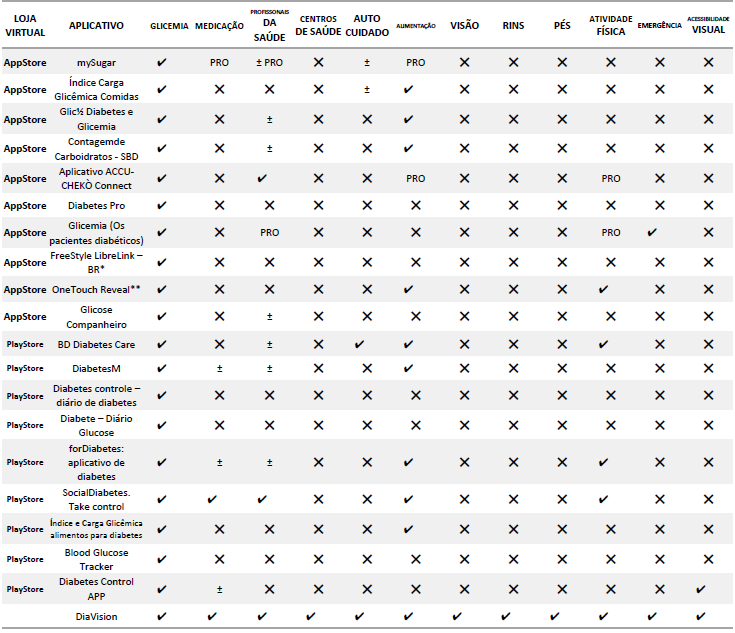
\includegraphics[scale=0.75]{Imagens/proposta/busca_anterioridade.png}
    \end{center}
    \legend{Fonte: \cite{Sobral2021}.}
\end{figure}

\newpage

\section{Visão e Análise}

Nesta seção são descritas as necessidades e características esperadas do produto de \emph{software} a ser desenvolvido, identificadas a partir de
reuniões com a dona do produto (PO, do inglês \emph{product owner}), esta que identificou a problemática abordada neste trabalho e
realizou o levantamento de funcionalidades e problemas das soluções já existentes no mercado em \citeonline{Sobral2021}.

\subsection{Descrição do Problema}

A \autoref{tab-desc-pro} apresenta, de forma resumida, o problema, seus impactos e a proposta de solução com seu diferencial.

\begin{table}[htb]
    \caption{Descrição do problema.}
    \label{tab-desc-pro}
    \begin{center}
        \begin{tabular}{p{4.0cm}|p{10.0cm}}
            \textbf{Problema}    & Dificuldade de acesso à informações de autocuidado com relação ao DM por deficientes visuais.                                          \\
            \hline
            \textbf{Afeta}       & Independência e qualidade de vida de diabéticos com DV\@.                                                                              \\
            \hline
            \textbf{Impacta}     & No autocuidado e, consequentemente, no controle do DM\@.                                                                               \\
            \hline
            \textbf{Solução}     & Desenvolvimento de aplicação móvel com conteúdos e funcionalidades que auxiliem diabéticos no gerenciamento do autocuidado com o DM\@. \\
            \hline
            \textbf{Diferencial} & Acessibilidade ao deficiente visual.
        \end{tabular}
    \end{center}
    \legend{Fonte: Autores.}
\end{table}

\subsection{Riscos e Impedimentos}

Os seguintes riscos e possíveis impedimentos com relação ao produto foram identificados:

\begin{itemize}
    \item Não adesão por parte do público alvo;
    \item Dificuldades no manuseio do \emph{smartphone} pelo público alvo;
    \item Dificuldade de localizar os possíveis participantes da pesquisa;
    \item Utilização incorreta do aplicativo ou não assimilação das informações adquiridas;
    \item Afastamento do paciente da assistência continuada na rede primária;
    \item Constrangimento do usuário por falta de entendimento das funcionalidades.
\end{itemize}

\newpage

\section{Requisitos}

Antes de inciar o desenvolvimento de qualquer tarefa técnica de engenharia de \emph{software}, é interessante que seja criado
um conjunto de requisitos.
Isso porque as tarefas de levantamento de requisitos levam a um entendimento dos impactos da solução, necessidades do cliente e
como os usuários finais vão interagir com o \emph{software}, diminuindo as chances de erros por má interpretação das solicitações
dos clientes \cite{pressman2014software}.

Esses requisitos costumam ser classificados como funcionais, não-funcionais e inversos \cite{sommerville2007engenharia}.
E serão apresentados nesta seção, iniciando pelas estórias de usuários, parte inicial do processo de elicitação
dos requisitos e finalizando com os casos de uso.

\newpage

\subsection{Estórias de usuários}

Estórias de usuários são muito utilizadas em metodologias ágeis e descrevem um cenário geral onde é possível visualizar
quais ações são possíveis, os atores envolvidos e quais os valores dessas ações, servindo como lembrete
de possíveis requisitos que precisam ser melhor detalhados com o cliente \cite{nawrocki2014agile}.

As estórias de usuários identificadas são listadas na \autoref{tab-est-usr}.

\begin{table}[htb]
    \begin{center}
        \ABNTEXfontereduzida
        \caption{Relação de estórias de usuários.}
        \label{tab-est-usr}
        \begin{tabular}{p{2.0cm}|p{5.0cm}|p{7.0cm}}
            %\hline
            \textbf{Eu, enquanto}                                          & \textbf{Quero} & \textbf{Para}                     \\
            \hline
            Paciente                                                       &
            Encontrar o \emph{app} nas lojas virtuais                      &
            Baixar o \emph{app} no meu celular.                                                                                 \\
            \hline
            Paciente                                                       &
            Realizar cadastro no aplicativo                                &
            Ter acesso às funcionalidades do \emph{app}.                                                                        \\
            \hline
            Paciente                                                       &
            Realizar login de forma prática                                &
            Para acessar as funcionalidades do \emph{app}.                                                                      \\
            \hline
            Paciente                                                       &
            Poder alterar minha senha                                      &
            Poder alterá\@-la e recuperar acesso ao \emph{app}.                                                                 \\
            \hline
            Paciente                                                       &
            Registrar informações das refeições                            &
            Acompanhar a quantidade de calorias consumidas por refeição.                                                        \\
            \hline
            Paciente                                                       &
            Ter acesso a aplicativos acessíveis para deficientes visuais   &
            Ajudar a realizar atividades do dia a dia.                                                                          \\
            \hline
            Paciente                                                       &
            Sugerir aplicativos acessíveis para deficientes visuais        &
            Compartilhar aplicativos que possam ajudar outros usuários com DV\@.                                                \\
            \hline
            Paciente                                                       &
            Registrar práticas de atividade física                         &
            Acompanhar a evolução da rotina de atividade física.                                                                \\
            \hline
            Paciente                                                       &
            Ter acesso à dicas de autocuidado                              &
            Melhorar a qualidade de vida e prevenir complicações do DM\@.                                                       \\
            \hline
            Paciente                                                       &
            Filtrar as dicas por categorias                                &
            Facilitar a busca das dicas sobre assuntos específicos.                                                             \\
            \hline
            Paciente                                                       &
            Consultar locais para acesso à serviços de saúde               &
            Facilitar o acesso e contato com as principais clínicas, hospitais e consultórios da cidade.                        \\
            \hline
            Paciente                                                       &
            Registrar glicemia                                             &
            Acompanhamento dos valores de glicemia e ser alertado quando estiver fora do limite.                                \\
            \hline
            Paciente                                                       &
            Registrar medicações que faço uso                              &
            Ter uma lista atualizada com todas as informações das medicações e ser alertado dos horários de uso das medicações. \\
            \hline
            Paciente                                                       &
            Realizar avaliação dos pés                                     &
            Acompanhar a evolução dos pés e detectar quando surgir alterações.                                                  \\
            \hline
            Paciente                                                       &
            Registrar diurese diária                                       &
            Acompanhar quando surgir alterações.                                                                                \\
            \hline
            Paciente                                                       &
            Ter acesso a relatórios dos dados registrados                  &
            Visualizar e compartilhar esses dados registrados.                                                                  \\
            \hline
            Paciente                                                       &
            Ter acesso aos dados pessoais                                  &
            Editar ou acrescentar dados pessoais durante o uso do aplicativo.                                                   \\
            \hline
            Paciente                                                       &
            Configurar notificações                                        &
            Definir horários e quais ativar ou desativar.                                                                       \\
            \hline
            Paciente                                                       &
            Configurar preferências                                        &
            Personalizar os limites da glicemia.                                                                                \\
            \hline
            Paciente                                                       &
            Realizar \emph{logout}                                         &
            Para desvincular minha conta do \emph{app}.                                                                         \\
            \hline
            Administrador do sistema                                       &
            Adicionar dicas de autocuidado para os pacientes               &
            Fornecer informações acerca de cuidados com a saúde.                                                                \\
            \hline
            Administrador do sistema                                       &
            Cadastrar centros de saúde no sistema                          &
            Que o paciente possa conhecer os centros de saúde que atendem suas demandas.                                        \\
            \hline
            Administrador do sistema                                       &
            Cadastrar sugestões de aplicativos acessíveis no sistema       &
            Que o paciente possa conhecer outros \emph{apps} acessíveis que possam ajudá\@-lo no cotiano.                       \\
            \hline
            Administrador do sistema                                       &
            Aprovar/recusar as sugestões de centros de saúde e aplicativos &
            Assegurar credibilidade ao aplicativo.                                                                              \\
            % \hline
        \end{tabular}
        \legend{Fonte: Autores.}
    \end{center}
\end{table}

\newpage

\subsection{Requisitos Funcionais}

A \autoref{tab-req-fun} mostra os requisitos funcionais da aplicação, estes que se referem, principalmente, às funções e 
comportamentos do sistema.

\begin{table}[htb]
    \begin{center}
        \ABNTEXfontereduzida
        \caption{Requisitos Funcionais da aplicação.}
        \label{tab-req-fun}
        \begin{tabular}{p{1.1cm}|p{1.3cm}|p{3.0cm}|p{1.5cm}|p{6.7cm}}
            %\hline
            \textbf{Código} & \textbf{Atores} & \textbf{Requisito}              & \textbf{Prioridade} & \textbf{Descrição} \\
            \hline
            RF01            & Paciente        & Manter paciente                 & Essencial           &
            O paciente poderá gerenciar seus dados na aplicação.                                                           \\
            \hline
            RF02            & Paciente        & Resetar senha                   & Essencial           &
            O paciente poderá solicitar a alteração de senha para recuperar acesso.                                        \\
            \hline
            RF03            & Paciente        & Autenticação                    & Essencial           &
            Será necessária autenticação com e-mail e senha para ter acesso às funcionalidades do \emph{app}.              \\
            \hline
            RF04            & Adminis-trador  & Manter Dicas de Autocuidado     & Essencial           &
            O administrador do sistema poderá gerenciar as dicas de autocuidado no sistema.                                \\
            \hline
            RF05            & Adminis-trador  & Manter Centros de Saúde         & Desejável           &
            O administrador do sistema poderá gerenciar os centros de saúde no sistema.                                    \\
            \hline
            RF06            & Adminis-trador  & Manter \emph{Apps} de Visão     & Importante          &
            O administrador do sistema poderá gerenciar sugestões de aplicativos acessíveis à PDV\@.                       \\
            \hline
            RF07            & Paciente        & Manter Registros de Diurese     & Importante          &
            O paciente poderá registrar diurese e gerenciar esses registros.                                               \\
            \hline
            RF08            & Paciente        & Manter Registros de Glicemia    & Essencial           &
            O paciente poderá registrar níveis de glicemia e gerenciar esses registros.                                    \\
            \hline
            RF09            & Paciente        & Manter Registros de Medicação   & Essencial           &
            O paciente poderá registrar suas medicações e gerenciar esses registros.                                       \\
            \hline
            RF10            & Paciente        & Manter Registros de Exercícios  & Importante          &
            O paciente poderá registrar atividades físicas realizadas e gerenciar esses registros.                         \\
            \hline
            RF11            & Paciente        & Manter Avaliações dos Pés       & Essencial           &
            O paciente poderá registrar avaliações do estado dos pés e gerenciar esses registros.                          \\
            \hline
            RF12            & Paciente        & Sugerir \emph{Apps} de Visão    & Importante          &
            O paciente poderá sugerir de aplicativos acessíveis à PDV para avaliação do administrador.                     \\
            \hline
            RF13            & Paciente        & Manter Registros de Alimentação & Essencial           &
            O paciente poderá registrar os alimentos que consumiu por refeição e gerenciar esses registros.                \\
            \hline
            RF14            & Paciente        & Consultar Dicas de Autocuidado  & Essencial           &
            O paciente poderá consultar as dicas de autocuidado disponíveis no sistema.                                    \\
            \hline
            RF15            & Paciente        & Consultar Centros de Saúde      & Desejável           &
            O paciente poderá consultar os centros de saúde disponíveis no sistema.                                        \\
            \hline
            RF16            & Paciente        & Consultar \emph{Apps} de Visão  & Importante          &
            O paciente poderá consultar sugestões de aplicativos acessíveis à PDV\@ disponíveis no sistema.                \\
            \hline
            RF17            & Paciente        & Sugerir Centros de Saúde        & Desejável           &
            O paciente poderá sugerir centros de saúde para avaliação do administrador.                                    \\
            \hline
            RF18            & Paciente        & Configurar Notificações         & Essencial           &
            O paciente poderá configurar quais notificações deseja receber e os horários.                                  \\
            \hline
            RF19            & Paciente        & Envio de Notificações           & Essencial           &
            Notificações deverão ser enviadas de acordo com as configurações definidas pelo paciente.                      \\
            % \hline
        \end{tabular}
        \legend{Fonte: Autores.}
    \end{center}
\end{table}

\newpage

\subsection{Requisitos Não-Funcionais}

Requisitos não-funcionais em sistemas podem ser descritos como atributos de qualidade, desempenho, segurança ou gerais, estes que podem
ser identificados a partir das necessidades do cliente mesmo que não tenham sido falados explicitamente \cite{pressman2014software}.

Assim, na \autoref{tab-req-nf}, são listados esses requisitos identificados juntamente com o tipo e a prioridade
de cada um deles para este projeto.

\begin{table}[htb]
    \begin{center}
        \ABNTEXfontereduzida
        \caption{Requisitos Não-Funcionais da aplicação.}
        \label{tab-req-nf}
        \begin{tabular}{p{1.1cm}|p{1.6cm}|p{3.0cm}|p{1.5cm}|p{6.7cm}}
            %\hline
            \textbf{Código} & \textbf{Tipo} & \textbf{Requisito}              & \textbf{Prioridade} & \textbf{Descrição} \\
            \hline
            RNF01           & Usabilidade   & Acessibilidade                  & Essencial           &
            Implementar as técnicas de acessibilidade para solucionar os principais problemas relacionados.              \\
            \hline
            RNF02           & Usabilidade   & Simplicidade                    & Essencial           &
            \emph{Interface} simples e intuitiva, mantendo apenas as informações necessárias na tela.                    \\
            \hline
            RNF03           & Usabilidade   & Buscas Ágeis                    & Desejável           &
            Facilitar buscas por meio de \emph{auto complete}.                                                           \\
            \hline
            RNF04           & Segurança     & Compartilhamento de Informações & Essencial           &
            Somente o próprio usuário terá acesso e poderá compartilhar suas informações.                                \\
            \hline
            RNF05           & Tecnologia    & Aplicação multiplataforma       & Desejável           &
            Deve-se utilizar de ferramentas que possibilitem a construção da aplicação para Android e iOS\@.             \\
            % \hline
        \end{tabular}
        \legend{Fonte: Autores.}
    \end{center}
\end{table}

\subsection{Requisitos Inversos}

Os requisitos listados na \autoref{tab-req-inv}, chamados inversos, se referem às restrições, condições que não devem ocorrer no sistema.

\begin{table}[htb]
    \begin{center}
        \ABNTEXfontereduzida
        \caption{Requisitos Inversos da aplicação.}
        \label{tab-req-inv}
        \begin{tabular}{p{1.1cm}|p{1.5cm}|p{10.5cm}}
            %\hline
            \textbf{Código} & \textbf{Prioridade} & \textbf{Descrição}         \\
            \hline
            RI01            & Essencial           &
            Um usuário não deve poder acessar recursos de outros.              \\
            \hline
            RI02            & Essencial           &
            Os usuários não devem ser notificados se não estiverem deslogados. \\
            \hline
            RI03            & Essencial           &
            O administrador do sistema não deve ter acesso aos dados dos usuários.
            % \hline
        \end{tabular}
        \legend{Fonte: Autores.}
    \end{center}
\end{table}

\newpage

\subsection{Casos de Uso}

De acordo com \citeonline{pressman2014software}, um caso de uso é caracterizado como um ``contrato de comportamento'' que define como
um ator utiliza um sistema para alcançar algum objetivo e descreve um cenário de uso de forma simples do ponto de vista desse ator.

A partir dos requisitos e estórias de usuários identificados, o diagrama de casos de usos da \autoref{fig_use_cas} foi elaborado.

\begin{figure}[htb]
    \caption{\label{fig_use_cas}Diagrama de casos de uso.}
    \begin{center}
        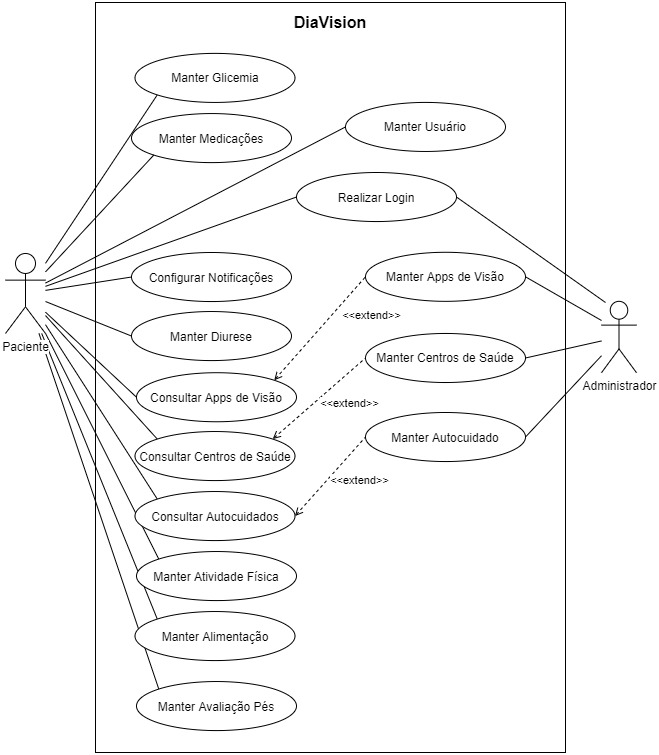
\includegraphics[scale=0.65]{Imagens/proposta/use_case.jpg}
    \end{center}
    \legend{Fonte: Autor.}
\end{figure}

\newpage

\section{Protótipo de Telas}

Nesta seção são apresentadas imagens do protótipo de telas elaborado no estudo \citeonline{Sobral2021}, com o objetivo de melhorar o entendimento dos
requisitos e funcionalidades do aplicativo que será desenvolvido.
Assim, nas \autoref{fig_tel_ini_prot} e \autoref{fig_tel_pos_prot} são mostradas as telas iniciais e demais telas do protótipo.

\begin{figure}[htb]
    \caption{\label{fig_tel_ini_prot}Telas iniciais do protótipo.}
    \begin{center}
        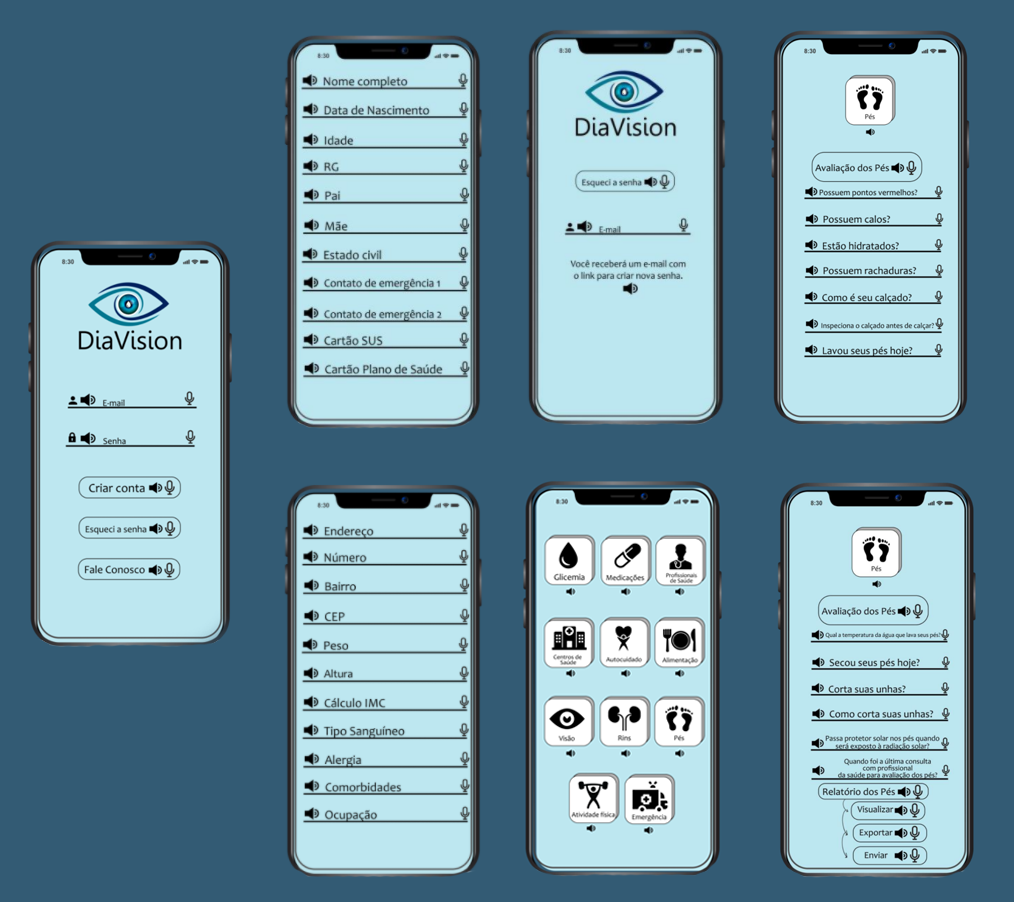
\includegraphics[scale=0.57]{Imagens/proposta/telas_iniciais_prot.png}
    \end{center}
    \legend{Fonte: \cite{Sobral2021}.}
\end{figure}

\begin{figure}[htb]
    \caption{\label{fig_tel_pos_prot}Demais telas do protótipo.}
    \begin{center}
        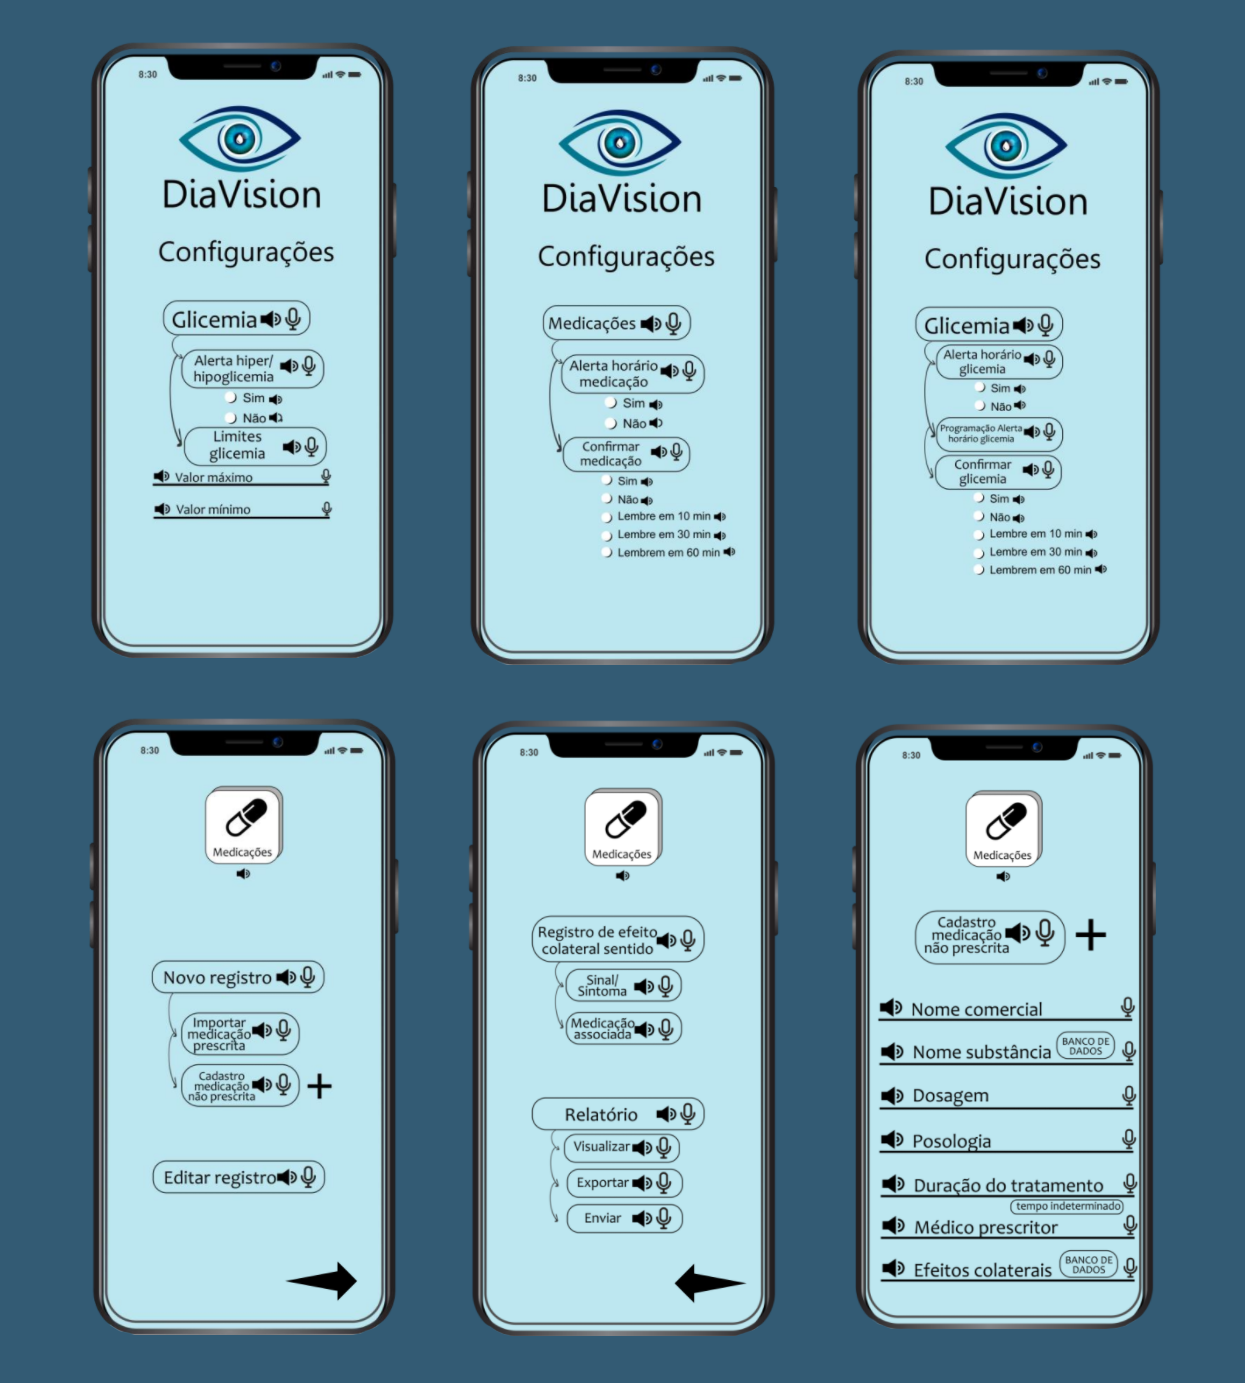
\includegraphics[scale=0.45]{Imagens/proposta/telas_post_prot.png}
    \end{center}
    \legend{Fonte: \cite{Sobral2021}.}
\end{figure}

\newpage

\section{Cronograma}

Por fim, o cronograma na \autoref{fig_cro_con} foi definido visando a organização e planejamento das atividades que serão realizadas
na segunda parte desse trabalho.

\begin{figure}[htb]
    \caption{\label{fig_cro_con}Cronograma de continuidade do Projeto.}
    \begin{center}
        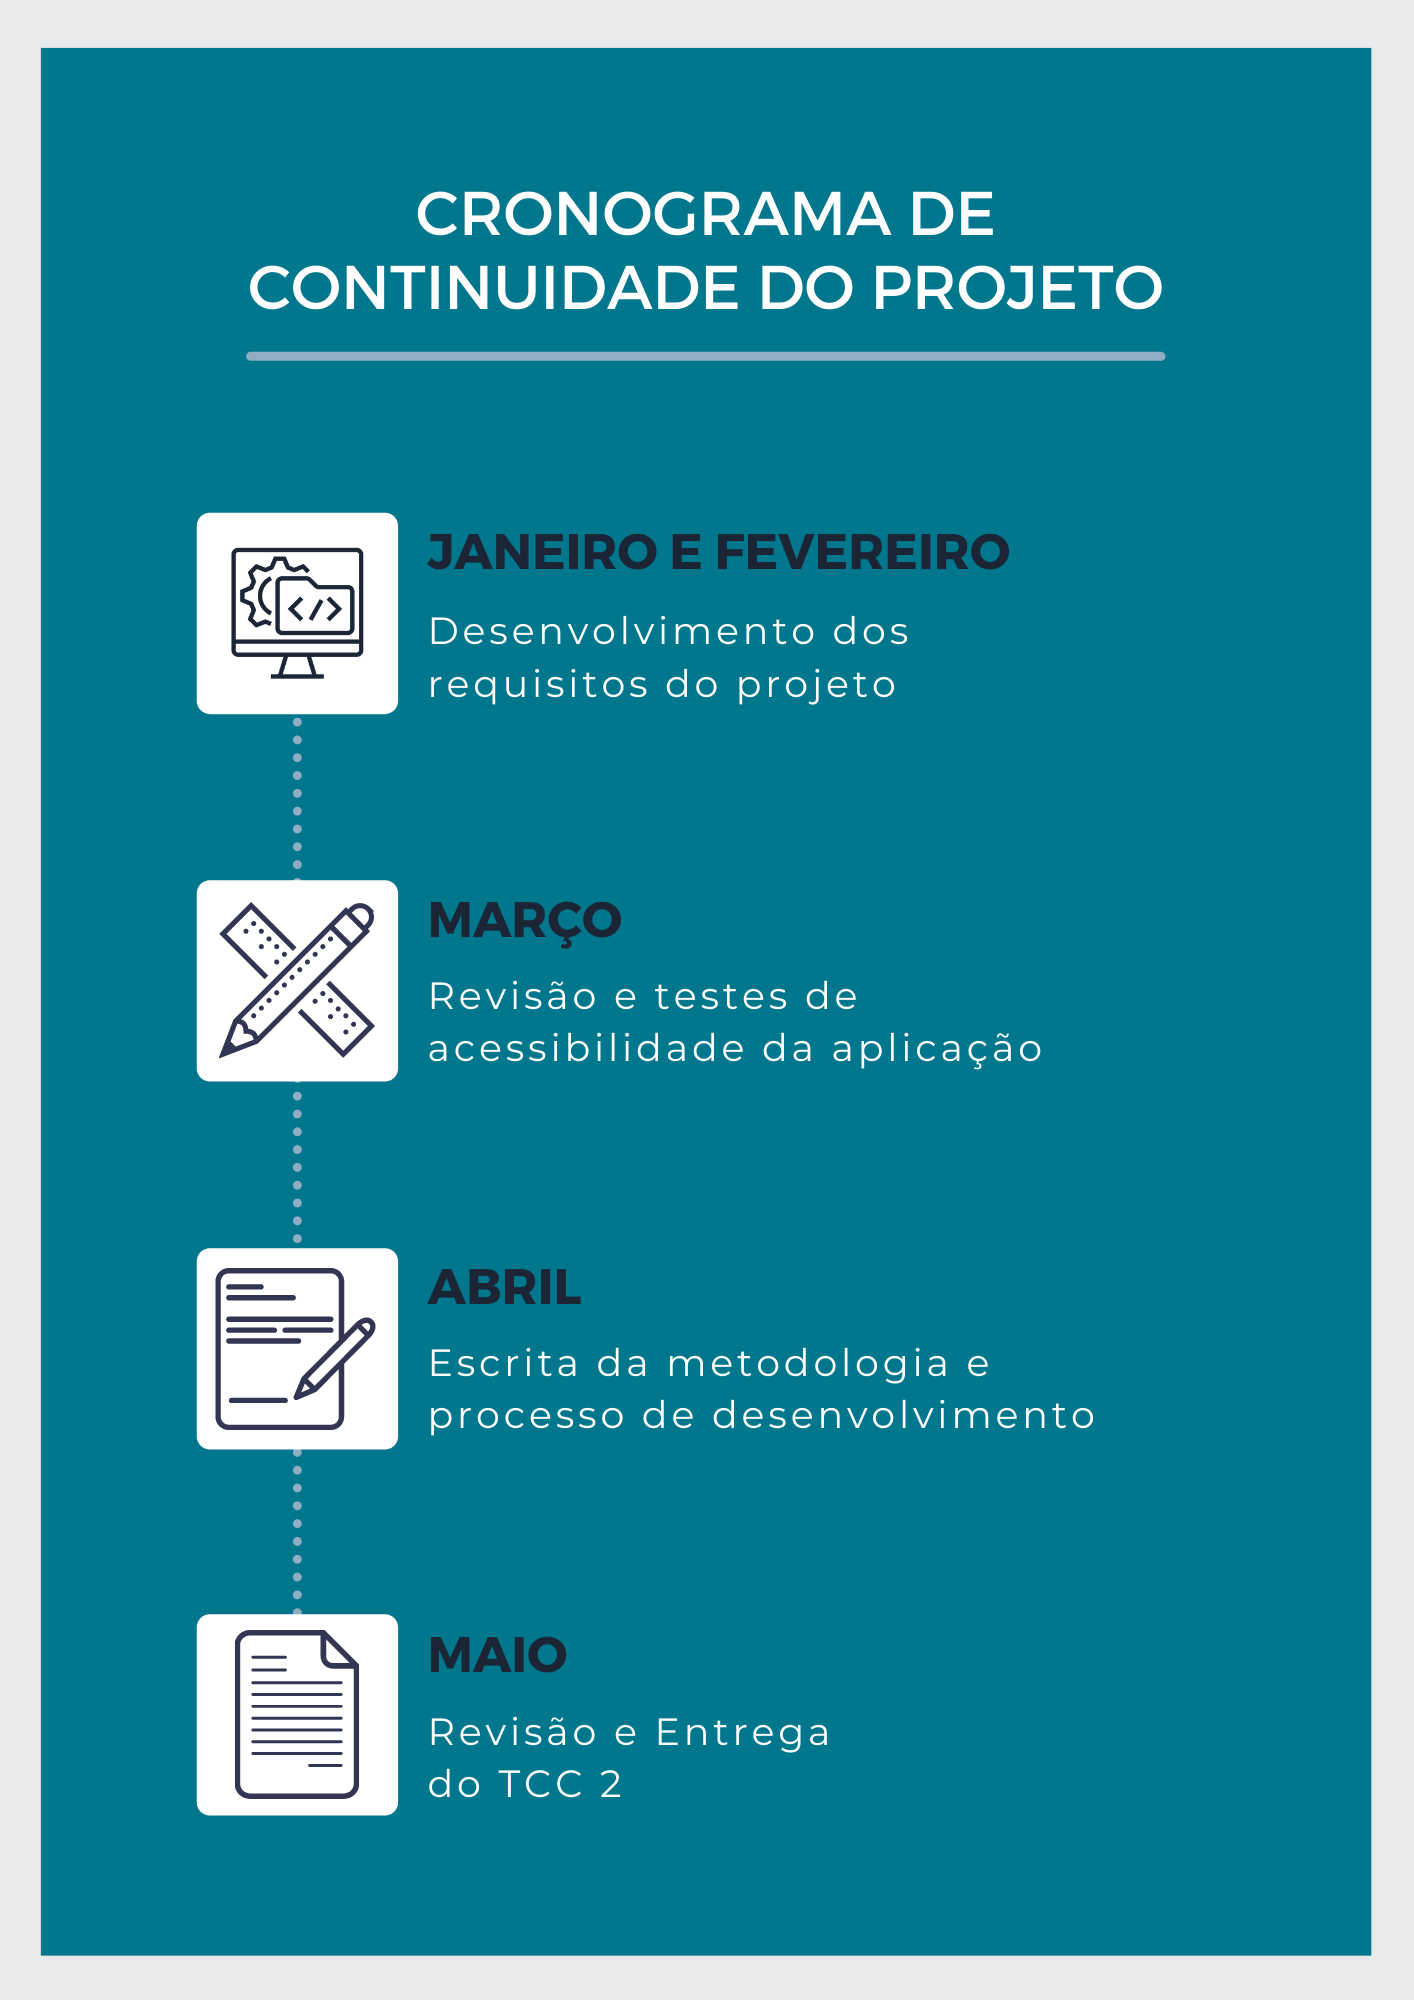
\includegraphics[scale=0.65]{Imagens/proposta/cronograma_continuidade.png}
    \end{center}
    \legend{Fonte: Autor.}
\end{figure}
% \chapter{Considerações Finais}
\label{ch:conclusion}

Este trabalho buscou contextualizar e fundamentar a problemática identificada pela dificuldade
no acesso à informações sobre o autocuidado com o DM por pacientes com DV\@. Para isso, foram introduzidos
o DM e suas complicações relacionadas à DV, bem como, foram apresentados dados que indicam o crescimento no
número de casos de ambos.

Por meio de estudos anteriores, em um trabalho de mestrado que acarretou na parceira para desenvolvimento deste
projeto, foi possível um aprofundamento sobre as necessidades e requisitos do público-alvo.
Onde foram identificadas a importância do autocuidado no tratamento do DM e as principais funcionalidades utilizadas
como solução no mercado \cite{Sobral2021}.

Outra problemática introduzida foi que, mesmo com o aumento da informatização e popularização dos \emph{smartphones},
PDV ainda enfrentam sérios problemas quanto à falta de acessibilidade à DV em aplicações móveis \cite{Shera2021285}.
E apontadas as principais ferramentas e diretrizes relacionadas à acessibilidade disponibilizadas pelas plataformas móveis.

Assim, foi realizado um processo de MSL visando identificar as principais soluções que estão sendo adotadas
para essa problemática. Nesse processo de mapeamento, foram extraídas informações relevantes
de trabalhos publicados em bases acadêmicas que apresentaram técnicas para resolver esses problemas
em aplicações móveis.

A partir da análise dos resultados do MSL, estabeleceram-se as técnicas de acessibilidade que seriam utilizadas
na solução proposta, sendo apresentados o planejamento e cronograma de continuidade de seu desenvolvimento.

Concluímos que o autocuidado pode ajudar a reduzir significativamente as complicações ocasionadas pelo DM \cite{ADA2019}.
Assim, aliando-o ao crescimento no acesso à Internet por meio de \emph{smartphones}, de acordo com \citeonline{CETIC_2021},
e à aplicação das principais técnicas para resolução dos problemas de acessibilidade em aplicativos móveis, propomos o
desenvolvimento de uma aplicação fruto da combinação de todas essas características.

\phantompart
\bibliography{Bibliografia}

%%%%%%%%%%%%%%%%%%%%%%%%%%%%%%%%%%%%%%%%%%%%%%%%%%%%%%%%%%%%%%%%%%%%%%%%%%
% ELEMENTOS PÓS-TEXTUAIS
%%%%%%%%%%%%%%%%%%%%%%%%%%%%%%%%%%%%%%%%%%%%%%%%%%%%%%%%%%%%%%%%%%%%%%%%%%

%\postextual

\renewcommand{\chapnumfont}{\chaptitlefont}
\renewcommand{\afterchapternum}{}
%\include{Pos_Textual/Apendices}
%\include{Pos_Textual/Anexos}

\end{document}